%%%%%%%%%%%%%%%%%%%%%%%%%%%%%%%%%%%%%%%%%%%%%%%%%%%%%%%%%%%%%%%%%%%%%%%%%%%%%%%%%%%%%%%%%%%%%%%%%%%%%%%%%%%%%%%%%%%%%%%%%%%%%%%%%%%%%%%%%%%%%%%%%%%%%%%%%%%
% This is just an example/guide for you to refer to when submitting manuscripts to Frontiers, it is not mandatory to use Frontiers .cls files nor frontiers.tex  %
% This will only generate the Manuscript, the final article will be typeset by Frontiers after acceptance.                                                 %
%                                                                                                                                                         %
% When submitting your files, remember to upload this *tex file, the pdf generated with it, the *bib file (if bibliography is not within the *tex) and all the figures.
%%%%%%%%%%%%%%%%%%%%%%%%%%%%%%%%%%%%%%%%%%%%%%%%%%%%%%%%%%%%%%%%%%%%%%%%%%%%%%%%%%%%%%%%%%%%%%%%%%%%%%%%%%%%%%%%%%%%%%%%%%%%%%%%%%%%%%%%%%%%%%%%%%%%%%%%%%%

%%% Version 3.1 Generated 2015/22/05 %%%
%%% You will need to have the following packages installed: datetime, fmtcount, etoolbox, fcprefix, which are normally inlcuded in WinEdt. %%%
%%% In http://www.ctan.org/ you can find the packages and how to install them, if necessary. %%%

%\documentclass{frontiersSCNS} % for Science, Engineering and Humanities and Social Sciences articles
%\documentclass{frontiersHLTH} % for Health articles
\documentclass{frontiersFPHY} % for Physics and Applied Mathematics and Statistics articles

%\setcitestyle{square}
\usepackage{url,hyperref,lineno,microtype}
\usepackage[onehalfspacing]{setspace}
\usepackage{textgreek}
\usepackage{xspace}
\usepackage{siunitx}
\linenumbers

\DeclareSIUnit\Molar{\textsc{M}}
\newcommand{\Ab}{A\textbeta\xspace}
\newcommand{\ie}{i.~e.\xspace}
\newcommand{\q}{\boldsymbol{q}}
\newcommand{\dd}{\partial}
\newcommand{\vect}[1]{\boldsymbol{#1}}
\newcommand{\Abs}{A\textbeta\textsubscript{1-40}\xspace}


% Leave a blank line between paragraphs instead of using \\


\def\keyFont{\fontsize{8}{11}\helveticabold }
\def\firstAuthorLast{Diem {et~al.}} %use et al only if is more than 1 author
\def\Authors{Alexandra K. Diem\,$^{1,*}$, Matthew MacGregor Sharp\,$^{2}$, Maureen Gatherer\,$^{2}$, Neil W. Bressloff\,$^{1}$, Roxana O. Carare\,$^{2}$ and Giles Richardson\,$^3$}
% Affiliations should be keyed to the author's name with superscript numbers and be listed as follows: Laboratory, Institute, Department, Organization, City, State abbreviation (USA, Canada, Australia), and Country (without detailed address information such as city zip codes or street names).
% If one of the authors has a change of address, list the new address below the correspondence details using a superscript symbol and use the same symbol to indicate the author in the author list.
\def\Address{$^{1}$Computational Engineering and Design, Faculty of Engineering \& the Environment, University of Southampton, Southampton SO16 7QF, UK \\
$^{2}$Clinical Neurosciences, Faculty of Medicine, University of Southampton, Southampton General Hospital, Southampton SO16 6YD, UK\\
$^{3}$Mathematical Sciences, Faculty of Social, Human and Mathematical Sciences, University of Southampton, Southampton SO17 1BJ, UK}
% The Corresponding Author should be marked with an asterisk
% Provide the exact contact address (this time including street name and city zip code) and email of the corresponding author
\def\corrAuthor{A.~K.~Diem}
\def\corrAddress{Computational Engineering and Design, Faculty of Engineering \& the Environment, University of Southampton, Southampton SO16 7QF, UK}
\def\corrEmail{A.K.Diem@soton.ac.uk}




\begin{document}
\onecolumn
\firstpage{1}

\title[Arterial pulsations cannot drive periarterial drainage]{Arterial pulsations cannot drive intramural periarterial drainage: Significance for \Ab drainage} 

\author[\firstAuthorLast ]{\Authors} %This field will be automatically populated
\address{} %This field will be automatically populated
\correspondance{} %This field will be automatically populated

\extraAuth{}% If there are more than 1 corresponding author, comment this line and uncomment the next one.
%\extraAuth{corresponding Author2 \\ Laboratory X2, Institute X2, Department X2, Organization X2, Street X2, City X2 , State XX2 (only USA, Canada and Australia), Zip Code2, X2 Country X2, email2@uni2.edu}


\maketitle

%%%%%%%%%%%%%%%%%%%%%%%%%%%%%%%%%%%%%%%%%%%%%%%%%%%%%%%%%%%%%%%%%%%%%%%%%%%%%%%%%%%%%%%%%%%%%%%%%%%%%%%%%%%%%%%%%%%%%%%%%%%%%%%%%%%%%%%%%%%%%%%%%%%%%%%%%%%%%%%%%%%%%%%%%%%%%%%%%%%%%%%%%%%%%%%%%%%%%%%%%%%%%%%%%%%%%%%%%%%%%%%%%%%%%%%
%%% The sections below are for reference only.
%%%
%%% For Original Research Articles, Clinical Trial Articles, and Technology Reports the section headings should be those appropriate for your field and the research itself. It is recommended to organize your manuscript in the
%%% following sections or their equivalents for your field:
%%% Abstract, Introduction, Material and Methods, Results, and Discussion.
%%% Please note that the Material and Methods section can be placed in any of the following ways: before Results, before Discussion or after Discussion.
%%%
%%%For information about Clinical Trial Registration, please go to http://www.frontiersin.org/about/AuthorGuidelines#ClinicalTrialRegistration
%%%
%%% For Clinical Case Studies the following sections are mandatory: Abstract, Introduction, Background, Discussion, and Concluding Remarks.
%%%
%%% For all other article types there are no mandatory sections.
%%%%%%%%%%%%%%%%%%%%%%%%%%%%%%%%%%%%%%%%%%%%%%%%%%%%%%%%%%%%%%%%%%%%%%%%%%%%%%%%%%%%%%%%%%%%%%%%%%%%%%%%%%%%%%%%%%%%%%%%%%%%%%%%%%%%%%%%%%%%%%%%%%%%%%%%%%%%%%%%%%%%%%%%%%%%%%%%%%%%%%%%%%%%%%%%%%%%%%%%%%%%%%%%%%%%%%%%%%%%%%%%%%%%%%%

\begin{abstract}

%%% Leave the Abstract empty if your article falls under any of the following categories: Editorial Book Review, Commentary, Field Grand Challenge, Opinion or specialty Grand Challenge.
  \section{
    Alzheimer's Disease (AD) is the most common form of dementia and to date there is no cure or efficient prophylaxis. The cognitive decline correlates with the accumulation of amyloid-\textbeta\xspace (\Ab) in the walls of capillaries and arteries. Our group has demonstrated that interstitial fluid and \Ab are eliminated from the brain along the basement membranes of capillaries and arteries, the intramural periarterial drainage (IPAD) pathway. With advancing age and arteriosclerosis, the stiffness of arterial walls, this pathway fails in its function and \Ab accumulates in the walls of arteries. In this study we tested the hypothesis that arterial pulsations drive IPAD and that a valve mechanism ensures the net drainage in a direction opposite to that of the blood flow. This hypothesis was tested using a mathematical model of the  drainage mechanism. We demonstrate firstly that arterial pulsations are not strong enough to produce drainage velocities comparable to experimental observations. Secondly, we demonstrate that a valve mechanism such as directional permeability of the IPAD pathway is necessary to achieve a net reverse flow. The mathematical simulation results are confirmed by assessing the pattern of IPAD in mice using pulse modulators, showing no significant alteration of IPAD. Our results indicate that forces other than the cardiac pulsations are responsible for efficient IPAD.
  }
%As a primary goal, the abstract should render the general significance and conceptual advance of the work clearly accessible to a broad readership. References should not be cited in the abstract.
%For full guidelines regarding your manuscript please refer to \href{http://www.frontiersin.org/about/AuthorGuidelines}{Author Guidelines} \\ or \textbf{Table \ref{Tab:01}} for a summary according to article type.


\tiny
 \keyFont{ \section{Keywords:} Alzheimer's disease; cerebral blood flow; perivascular drainage; intramural periarterial drainage; cerebral lymphatics } %All article types: you may provide up to 8 keywords; at least 5 are mandatory.
\end{abstract}

\section{Introduction}

Alzheimer's disease (AD) is the commonest form of dementia. Although it has been studied for over 100 years \cite{Selkoe2001}, to date there is no cure as the processes relevant to its onset and progression have not yet been fully understood. The pathology of AD comprises the degeneration and death of neurons, synapse loss, neuroinflammation and the intracellular as well as extracellular accumulation of proteins \cite{Koffie2011}. The protein amyloid-\textbeta\xspace (\Ab) is produced as part of the normal metabolism of healthy brains, but it plays a major role in the development of AD \cite{Haass1992}. According to the \Ab hypothesis AD is caused by a failure to remove \Ab from the brain and successively, its accumulation in the form of plaques in the parenchyma. Prior to the buildup of plaques in the brain \Ab accumulates in the walls of cerebral blood vessels as cerebral amyloid angiopathy (CAA), which correlates much better with the degree of dementia compared to the number and size of plaques and appears in \SIrange{90}{96}{\percent} of AD patients \cite{Weller2006, Weller2009}.

In order to process metabolites, the brain requires a lymphatic system that transports waste products to the lymph nodes, where they are decomposed. While the rest of the body possesses a dedicated network of lymphatic vessels these do not exist in the brain \cite{Weller2010}. Both the pathology of CAA and ample evidence from injection studies suggest that the basement membranes (BM) in the walls of cerebral arteries provide the clearance pathway for interstitial fluid (ISF) towards the surface of the brain, also referred to as intramural periarterial drainage (IPAD) \cite{Weller2010,Carare2008,Hawkes2011,Morris2014}. It is important not to confuse the IPAD pathway with the Virchow-Robin spaces, which are often referred to as perivascular (or ``paravascular'') spaces, possibly artefactual, located between the glia limitans and the arterial wall. Virchow-Robin spaces are virtual spaces and have no role in \Ab drainage. The BM forming the IPAD does not actually constitute a space, but rather a fluid-filled protein matrix. Our understanding of the mechanism that drives perivascular drainage through the BM is still very limited. The evidence indicates that ISF enters the BM at the capillary level and flows towards the lymph nodes in the neck via the BM cerebral arteries. This suggests that the counterintuitive phenomenon of ISF flow occurs in the reverse direction to blood flow \cite{Carare2008}.

A widely accepted hypothesis for the driving mechanism of this reverse perivascular drainage of solutes from the brain is that it is driven by arterial pulsations \cite{Weller2009,Carare2008,Hawkes2011,Morris2014,Schley2006,Attems2011,Wang2011,Iliff2012,Asgari2015,Sharp2015,Weller2015a}. In this paper we tested this hypothesis by using a multi-scale modelling approach combining analytical and numerical methods. The BM is modelled as a porous medium using a lubrication approximation. Flow inside the BM is driven by both the ISF pressure gradient and the deformation of the arterial wall, which are obtained from a numerical model of the middle cerebral artery (MCA). To give IPAD in the reverse direction to the blood flow, a valve mechanism is required; here it is modelled by a pressure gradient dependent permeability. It is shown that this valve mechanism is necessary to achieve net reverse drainage. However, due to the long wavelength of arterial pulsations the pressure gradients inside the BM are too small to drive fluid flow at the expected velocities. The resulting velocity of the model was at least four orders of magnitude smaller than values obtained experimentally \cite{Carare2008}. Therefore, arterial pulsations are concluded to be insufficient to drive perivascular drainage along the BM of cerebral arteries. The simulation results are confirmed by an experimental assessment of the effect of pulse modulation in a mouse model, which showed no significant difference in IPAD compare to control mice.

%\begin{methods}
\section{Numerical modelling of perivascular drainage of \Ab}

First, IPAD under a pressure-pulse driven scenario is evaluated using computational modelling. An analytical model of the BM was developed, which captures the preference of flow in the reverse direction to the blood flow. Pressure inside the BM is evaluated using a numerical model of blood pressure inside the artery and a stress analysis in the artery wall. These were then used to evaluate the velocity of perivascular drainage through the MCA.

\subsection{Porous medium model of lymphatic drainage through the BM}
\label{sec:diodemodel}

We propose a model of lymphatic drainage from the brain via the cerebral BM based on Darcy's law for flow in porous media. By exploiting the discrepancy of scales between the width of the BM and its length we approximate the flow by a one-dimensional lubrication model (see for example \cite{Ockendon1995}). Furthermore, we allow the permeability of the BM to depend on the pressure gradient of the ISF. Such a pressure gradient dependent permeability could, for instance, model proteins in the BM protein network that have structural properties that allow them to bend easily only in one direction, thereby acting as a valve, and thus provide a higher resistance to flow in the direction of the blood flow. A similar idea has been investigated in \cite{Sharp2015}, where proteins were explicitly modelled as cilia. However, here we model the active component of the BM generically in this model and thus allow for alternative explanations of the phenomenon.

The BM consists of a complex matrix of proteins (extracellular matrix, ECM) that can be interpreted as a porous medium through which soluble metabolites drain via the ISF. We model flow through this medium, in the standard fashion, by Darcy's law in a 2D cylindrical coordinate system. Darcy's law states that the flux $\q$ is related to the fluid pressure gradient $\boldsymbol{\nabla} p$ by
\begin{equation}\label{eq:darcy}
  \q = -\frac{k}{\mu} \boldsymbol{\nabla} p
\end{equation}
where $k$ is the intrinsic permeability of the ECM and $\mu$ is the viscosity of ISF. Since ISF flows up the artery, counter to the direction of arterial pulsations, a valve-like mechanism in the ECM is required if arterial pulsations are indeed the motive force for this flow. This valve-like property of the ECM can be modelled by a Darcy flow \eqref{eq:darcy}, in which the intrinsic permeability is a function of the axial pressure gradient $\dd p / \dd z$ along the vessel. On assuming an artery aligned along the $z$-axis with net blood flow and arterial pulsations propagating the positive $z$-direction we model valve-like properties of the ECM in the BM by a pressure gradient dependent permeability
\begin{equation}
k = \mu K(p_z) \qquad \text{where } p_z = \frac{\dd p}{\dd z}.
\end{equation}
In order to obtain a net flux up the vessel, counter to the blood flow, we require this function to be increasing in $p_z$, representing the notion that it is harder to push a flow in the positive $z$-direction ($p_z < 0$ and $K(p_z)$ small) than in the negative $z$-direction ($p_z \geq 0$ and $K(p_z)$ large).

The governing equations in cylindrical coordinates are thus
\begin{gather}
  \q = q_1 \vect{e_z} + q_2 \vect{e_r} = - K(p_z) \left( \vect{e_z} p_z + \vect{e_r} p_r \right) \label{eq:darcy_velocity}\\
  \frac{\dd q_1}{\dd z} + \frac{1}{r} \frac{\dd}{\dd r} \left( r q_2 \right) = 0 \label{eq:continuity},
\end{gather}
where $\vect{e_z}$ and $\vect{e_r}$ describe the unit vectors in the $z$ and $r$ direction. Incompressibility of the fluid is represented by \eqref{eq:continuity}.

To determine the boundary conditions of the system consider the geometry in Figure \ref{fig:pvs_model}. Under the assumption that the vessel deformations are radially symmetric the positions of the inner and outer sheaths bounding the BM can be described by the two expressions $r = R_i(z,t)$ and $r = R_o(z,t)$, respectively. Assuming that the flows through the surfaces of the BM are negligible the following kinematic boundary condition applies
\begin{equation} \label{eq:kinematic}  
\frac{D}{D t} \left( r - R_i(z,t) \right) = 0 \quad \text{on } r = R_i(z,t)
\end{equation}
and analogously for $R_o(z,t)$.

Because the BM thickness is much smaller than the vessel length it is possible, on using the lubrication approximation, to derive a 1D model (in $z$) for the BM thickness $h_\textrm{bm}(z,t)$; this takes the form
\begin{equation}
\begin{split}
\frac{\dd}{\dd t} \left( \gamma R_i(z,t) \cdot h_\textrm{bm}(z,t) \right) &=\\
\frac{\dd}{\dd z} \left( R_i(z,t) \right. & \left. \cdot h_\textrm{bm}(z,t) \cdot K(p_{z}) \cdot p_{z} \right),\label{eq:pvs_model}
\end{split}
\end{equation}
where $\gamma$ is the fluid volume fraction in the BM (see also SI~1). Equation \eqref{eq:pvs_model} describes the evolution of the BM thickness and can be solved using a finite difference approximation. For a detailed derivation see SI~1. Another method to arrive at the same equation is derived by considering an infinitesimally small volume of BM $dV = 2\pi \cdot R_i(z,t) \cdot h_\textrm{bm}(z,t) \cdot dz$. Then the difference between the flux into and out of the element $dV$ is equal to the rate of change of the fluid volume $\dd (\gamma dV)/ \dd t$, which can be written as
\begin{equation}
\begin{split}
\frac{\dd}{\dd t} \left( \gamma R_i(z,t) \cdot h_\textrm{bm}(z,t) \cdot dz \right) &=\\
& R_i(z,t) \cdot h_\textrm{bm}(z,t) \cdot q_1(z,t) -\\
R_i(z + dz,t) & \cdot h_\textrm{bm}(z + dz,t) \cdot q_1(z + dz,t),
\end{split}
\end{equation}
which is equal to the model equation \eqref{eq:pvs_model} in the limit $dz \rightarrow 0$. The pressure $p(z,t)$ and the displacement of the BM wall $R_i(z,t)$ are, to a very good approximation, determined solely by arterial pressure (\ie almost independent of the BM flow), see SI~2 for more details. $R_i(z,t)$ and $p_z$ are obtained from a numerical artery model described in the next section. To model the protein valve that is being proposed here, $K(p_z)$ is defined as a step function
\begin{equation}
  K(p_z) = \begin{cases}
    K_0 & p_z < 0\\
    K_1 & p_z \geq 0,
  \end{cases}
\end{equation}
such that $K_1 > K_0 > 0$ so that the BM is more permeable to ISF flow in the negative $z$-direction than in the positive one.

\subsection{Numerical Model of a Straight Arterial Section}


\begin{table}[!t]
\textbf{\refstepcounter{table}\label{tab:geometry} Table \arabic{table}.}{ Geometry parameters of the MCA section modelled using VaMpy \cite{Diem2016a}. }
\processtable{ }
             {\begin{tabular}{ccccl}\toprule
& MCA & left daughter & right daughter & \\
&     & vessel        & vessel         & \\
\midrule
$R_u$ & \SI{0.14}{\centi\metre} & \SI{0.13}{\centi\metre} & \SI{0.13}{\centi\metre} & upstream radius \\
$R_d$ & \SI{0.14}{\centi\metre} & \SI{0.08}{\centi\metre} & \SI{0.08}{\centi\metre} & downstream radius \\
$L$ & \SI{7}{\centi\metre} & \SI{6.5}{\centi\metre} & \SI{6.4}{\centi\metre} & length\\
\botrule
\end{tabular}}{}
\end{table}

\begin{table}[!t]
\textbf{\refstepcounter{table}\label{tab:simulation} Table \arabic{table}.}{ Simulation parameters for modelling a bifurcation of the MCA using VaMpy \cite{Diem2016a}. }
\processtable{ }
             {\begin{tabular}{ccc}\toprule
Parameter & Value & Physical meaning\\
\midrule
$k_1$ & \SI{2.0e7}{\gram\per\centi\metre\per\square\second} & wall elasticity \\
$k_2$ & \SI{-22.53}{\per\centi\metre} & parameters, \\
$k_3$ & \SI{8.65e5}{\gram\per\centi\metre\per\square\second} & see \eqref{eq:ehr} \cite{Olufsen2000,Diem2016a} \\
$\nu$ & \SI{0.046}{\square\centi\metre\per\second} & kinematic viscosity of blood\\
$R_1$ & \SI{14130}{\gram\per\centi\metre\tothe{4}\per\second} & First resistance element\\
$R_2$ & \SI{7200}{\gram\per\centi\metre\tothe{4}\per\second} & Second resistance element\\
$C_T$ & \SI{2.4752e-3}{\centi\metre\tothe{4}\square\second\per\gram} & Compliance element\\
$T$ & \SI{0.85}{\second} & cardiac cycle length\\
$t_c$ & 4 & number of cardiac cycles\\
$\Delta t$ & \SI{1e-5}{\second} & time step size\\
$\Delta z$ & \SI{0.1}{\centi\metre} & spatial step size\\
\botrule
\end{tabular}}{}
\end{table}

In order to obtain the input functions $R_i(z,t)$ and $p_z$ for the analytical model developed in the previous section, a section of human MCA was modelled as a 1D axisymmetric tube in a cylindrical coordinate system with cross-sectional lumen area $A(z,t)$ and flux $Q(z,t)$ using the Python package VaMpy \cite{Diem2016a}. The geometry parameters are listed in Table~\ref{tab:geometry}. Blood flow through arteries and the propagation of arterial pulsations are commonly described by a one-dimensional averaged model \cite{Olufsen2000} (for more details see \cite{Diem2016}). It is represented by the conservation law
\begin{equation}
  \frac{\dd \boldsymbol{U}}{\dd t} + \frac{\dd \boldsymbol{F}}{\dd z} = \boldsymbol{S}, \label{eq:conservation}
\end{equation}
where
\begin{gather*}
  \boldsymbol{U} = \begin{pmatrix} A(z,t) \\ Q(z,t) \end{pmatrix}, \quad \boldsymbol{F} = \begin{pmatrix} Q(z,t)\\ \dfrac{Q(z,t)^2}{A(z,t)} + f(r_0) \sqrt{A_0(z) A(z,t)} \end{pmatrix}, \quad \boldsymbol{S} = \begin{pmatrix} 0\\ S_1 \end{pmatrix}\\
S_1 = - \frac{2 \pi R(z,t)}{\delta_b \mathrm{Re}} \frac{Q(z,t)}{A(z,t)} + \left( 2 \sqrt{A(z,t)} \left( \sqrt{\pi} f(r_0) + \sqrt{A_0(z)} \frac{df(r_0)}{dr_0 } \right) - A(z,t) \frac{df(r_0)}{dr_0} \right) \frac{dr_0(z)}{dz}.
\end{gather*}
The equation is solved for cross-sectional area $A(z,t)$ of the vessel lumen and flux through the vessel $Q(z,t)$, where $R(z,t) = (A(z,t)/\pi)^{1/2}$ is the lumen radius, $\delta_b$ is the boundary layer thickness and $\text{Re}$ is the Reynolds number. Elasticity of the artery wall is modelled via the quantity $f(r_0) = 4Eh/(3r_0)$, where $E$ is the Young's modulus and $h$ is the wall thickness and $r_0(z)$ is the radius at rest. The relationship $Eh/r_0$ is based on compliance estimates
\begin{equation}
  \frac{Eh}{r_0} = k_1 \exp \left( k_2 r_0(z) \right) + k_3\label{eq:ehr}
\end{equation}
with $k_1, k_2, k_3$, see Table~\ref{tab:simulation} \cite{Olufsen2000}. Blood pressure $p(z,t)$ is related to $A(z,t)$ and $f(r_0)$ via the state equation
\begin{equation}
  p(z,t) - p_0 = f(r_0) \left( 1 - \frac{A_0(z)}{A(z,t)} \right),
\end{equation}
where $p_0$ is the diastolic pressure and $A_0(z)$ is the lumen radius at rest. Blood pressure provides the basis for determining ISF pressure inside the BM via the calculations in SI~2.

To derive \eqref{eq:conservation} it was necessary to make assumptions about the velocity profile of blood flow through an artery. Blood flow is considered pulsatile laminar and vessels are considered slightly tapered, therefore the velocity profile is assumed to be mostly flat with a thin boundary layer $\delta_b = (\nu T/(2\pi))^{0.5}$, such that $\delta_b \ll R(z,t)$ \cite{Olufsen2000}.

This system of equations can be solved numerically using Richtmyer's two-step version of the Lax-Wendroff method, as done by others \cite{Olufsen2000,LeVeque1992,Kolachalama2007}. We use the Python module from \cite{Diem2016a} to implement a model of the MCA and its first bifurcation. All simulation parameters are listed in Table~\ref{tab:simulation}. The MCA geometry data was taken from \cite{Cousins2014}, estimating lengths by $50 \cdot R_u$. The radii of the daughter vessels were estimated using a scaling factor of 0.91 \cite{Cousins2014}. The length of the right daughter vessel was shortened slightly to avoid reflective waves cancelling one another out \cite{Kolachalama2007}. A three-element Windkessel (3WK) model is used at the outlet whose parameters were obtained from \cite{Olufsen2002}.

At the inlet flux is prescribed using patient-specific flow velocity measurements collected from the MCA of a healthy adult male using Doppler Sonography ultrasound. The velocity data was converted to volumetric flux values within the range reported in \cite{Olufsen2002}. To obtain a smooth inlet function the final ten peaks of the time series were averaged in the Fourier space. The resulting inlet boundary condition is shown in Figure~\ref{fig:inlet}.

\subsection{IPAD through the MCA}

In the previous sections the models governing blood flow through the MCA and ISF flow through the artery wall have been introduced. Here, the results of the previous sections are coupled and used to calculate ISF flow through the BM with and without a valve mechanism to show its necessity to achieve net reverse drainage. At the same time it is shown that blood pressure driven perivascular drainage is far too slow to provide any meaningful flow, thereby disproving the popular hypothesis that arterial pulsations provide the major driving force for perivascular drainage. MCA simulations were run for eight cardiac cycles to allow the system to settle. An averate human heartbeat lasts \SI{0.85}{\second} and the total simulation time was \SI{6.8}{\second} (see Table~\ref{tab:simulation}). In the results presented here only the final heartbeat is shown. Figure~\ref{fig:mca} shows blood pressure (a), wall displacement (b) and ISF pressure (c) in the MCA. Because the radius of the MCA is very small its wall stiffness is high. Pressure gradients in time are therefore steep. This data provides the basis for estimating perivascular drainage through the cerebral vasculature.

Figure~\ref{fig:mca}b shows the displacement of the artery wall due to the pressure pulse. To calculate the width of the BM using the model equation \eqref{eq:pvs_model}, the input function $R_i(z,t)$ is the sum of the radius at rest and the wall displacement, as depicted in Figure~\ref{fig:pvs_model}. Figure~\ref{fig:h}a shows the width of the BM $h_\textrm{bm}(z,t)$ as calculated from \eqref{eq:pvs_model} over the length of the artery at a number of time points, while Figure~\ref{fig:h}b shows $\partial h_\textrm{bm}(z,t)/ \partial z$ for the same time points. The BM width only varies minimally around its initial width and thus flow rates of ISF are very small.

The results show that a valve mechanism is required to drive perivascular drainage in the reverse direction of the blood flow with an average flux of \SI{-1.12e-3}{\cubic\micro\metre\per\second} for a ratio of $K_0/K_1 = 0.01$, while it is \SI{6.33e-2}{\cubic\micro\metre\per\second} for $K_0/K_1 = 1.0$. While the results confirm the necessity of a strong valve mechanism under pulse driven flow they also indicate that arterial pulsations have too long a wavelength to drive significant perivascular drainage. Drainage velocity is fastest without a valve mechanism (\SI{1.81e-2}{\micro\metre\per\second}, and then it is in the wrong direction), but even in that case it is almost three orders of magnitude slower than the expected value of \SI{8.33}{\micro\metre\per\second} \cite{Carare2008}. The valve mechanism only guarantees net reverse drainage for a permeability ratio $K_0/K_1 < \SI{2.74e-2}{}$, where $K_1$ is chosen such that $k = \SI{1e-10}{\square\centi\metre}$ is consistent with values for other tissues in the body and $\mu = \SI{1.5e-3}{\pascal\second}$ \cite{Heppell2013}. Figure~\ref{fig:valve_test} illustrates flux through the BM for a number of ratios $K_0/K_1$ and for different positions of the BM $r = r_0 + \eta h$. Reverse flow is achieved for $K_0/K_1 < \SI{2.74e-2}{}$. Drainage flux values are fastest when the BM is placed close to the arterial lumen ($\eta = 0$) due to the elasticity of the artery wall.

The minute flux values are a result of the very small variations in BM width (see Figure~\ref{fig:h}) over the length of the MCA, in fact they are less than \SI{1}{\angstrom}. This value is far too small to be realistic and demonstrates that arterial pulsations cannot be strong enough to drive perivascular drainage through the BM. To illustrate it in another way, the total ISF volume in a human brain is \SI{280}{\milli\litre} \cite{Weller2015a}. At a drainage rate of \SI{-1.12e-3}{\cubic\micro\metre\per\second} per cerebral artery the total turnover time for ISF would be \SI{4.83e11}{} days, much more than a human life span.

\section{Experimental assessment of intramural perivascular drainage of \Ab}

In addition to performing simulations to assess the feasibility of arterial pulsations providing the main driving mechanism for IPAD, mouse model experiments were performed to confirm the results \textit{in vivo}. Experiments on mice were carried out on ten week old wild-type C57B16 mice ($n = 4$). All mice were kept on a standard \SI{12}{\hour} light/dark cycle and allowed food and water \textit{ad libitum}. All experiments were carried out in accordance with animal care guidelines stipulated by the Animal Care and Use Committee at the University of Southampton and the Home Office (PPL 20/2095).

To minimise the effects of anaesthesia on mouse cardiovascular function, isoflurane was chosen as the anaesthetizing agent. To reduce arterial pulsations, the beta-blocker Atenolol (Ate, \SI{10}{\milli\gram\per\kilo\gram}) was administered intraperitoneally (IP). Mouse vital parameters were monitored throughout the procedure using a MouseOX Plus and an infrared mouse thigh sensor (STARR Life Science, Holliston, MA, USA). Thermal regulation was maintained using a heat pad and rectal probe (BASi, West Lafayette, IN, USA). All intracerebral injections were performed using a \SIrange{1}{5}{\micro\litre} Hirschmann microcapillary pipette (Sigma UK) with a tip adjusted to a diameter of $<$ \SI{50}{\micro\metre} using a Sutter P97 Flaming Brown Pipette puller.

Mice were anaesthesized with isoflurane, placed prone on a stereotaxic instrument and secured with head adaptors. Baseline measurements of oxygen saturation, heart rate, breath rate and pulse distension were taken before administering Ate. A volume of \SI{0.5}{\micro\litre} of \Ab$_{1-40}$ HiLyte Fluor 555 (Cambridge Bioscience, UK) was stereotaxically injected into the left hippocampus at a rate of \SI{0.2}{\micro\litre\per\minute} (coordinates from Bregma: AP = \SI{-1.9}{\mm}; ML = \SI{1.5}{\mm} and DV = \SI{-1.7}{\mm}). Injection pipettes were left \textit{in situ} for \SI{2}{\minute} to prevent reflux. Mice were euthanized \SI{5}{\minute} after withdrawal of the injection pipette through overdose with pento-barbital (\SI{200}{\milli\gram\per\kilo\gram}). Mice were then intracardially perfused with \SI{0.01}{\Molar} phosphate buffered saline (PBS), pH 7.2 followed by \SI{4}{\percent} paraformaldehyde in \SI{0.01}{\Molar} PBS, pH 7.2. Brains were removed, post fixed overnight in fresh fixative and then processed for immunohistochemistry and image analysis. For controls, ten week old wild-type C57B16 mice were processed following the same method, but without the administration of Ate ($n = 3$). Detailed materials and methods can be found in SI~3.

\subsection{Immunohistochemistry}

Brains were cut into \SI{20}{\micro\metre} coronal sections using a freezing microtome (Leica) and the injection site located by examining on a Zeiss Axioskop 2 fitted with a rhodamine filter. Sections of \SI{400}{\micro\metre} and \SI{800}{\micro\metre} thickness both posterior and anterior to the injection site were selected for immunohistochemistry. Sections were blocked in \SI{15}{\percent} goat serum (Sigma 9023) for \SI{1}{\hour} at room temperature (RT). They were then incubated in primary antibodies diluted in \SI{0.01}{\Molar} phosphate buffered saline \SI{0.1}{\percent} triton x100 (PBSt). Primary antibodies comprised rabbit anti-collagen IV (AbCam, ab6586) 1/400 and mouse anti-smooth muscle actin (SMA) FITC conjugated (Sigma F3777) 1/200. Sections were incubated overnight at \SI{4}{\celsius} in a moist chamber. Following washing 3x \SI{10}{\minute} \SI{0.01}{\Molar} PBS sections were incubated in goat anti-rabbit Alexa Fluor 633 (ThermoFisher Scientific A-21070) 1/200 PBSt.

\subsection{Image Analysis}

Images of the whole hippocampus were captured on a Leica SP8 confocal microscope fitted with LASX software in tile scanning mode with sequential imaging. Once captured, images were exported as TIFF files and uploaded into Adobe Photoshop CS6. An area of hippocampus was drawn extending transversely from CA3 pyramidal cells to the apex of the blades of the granule cell layer and from the ventricle to \textit{stratum oriens} in the superior/inferior axis. \Ab containing vessels were defined according to size and presence of SMA: capillaries had a diameter of $\leq$ \SI{10}{\micro\metre}, veins had no SMA and a diameter of $>$ \SI{10}{\micro\metre}. The number of vessels was expressed per \SI{}{\square\milli\metre} of hippocampus. Statistical analysis was performed by an independent t-test with a confidence interval of \SI{95}{\percent}.

\subsection{Results}

Within \SI{5}{\minute} of injections into the hippocampus, fluorescent \Ab was observed diffusely in the hippocampus and co-localising with collagen IV with collagen IV in the walls of capillaries and arteries, with very few veins involved in both Ate-treated and control mice (Figure~\ref{fig:confocal}). Application of an independent t-test to the data revealed no significant differences between the saline and Ate treated mice either anterior or posterior to the injection site (Figure~\ref{fig:graph}).  

\section{Discussion and Conclusion}

The results show that the valve mechanism as implemented in our analytical model of the BM guarantees net reverse flow inside the BM under physiological blood flow conditions. The valve mechanism is required to be strong, \ie with a small ratio $K_0/K_1$, and necessary for net reverse flow to occur within the BM. This result agrees with previous modelling approaches that did not achieve net reverse drainage \cite{Schley2006,Wang2011}. The velocity of drainage additionally depends on the distance of the BM from the artery lumen. The closer the BM is placed to the lumen the faster net reverse drainage is, but variations remain within the same order of magnitude. This is due to the relatively large thickness of cerebral artery walls and their elastic properties. The hypothesis that the BM utilises a unidirectional valve mechanism is plausible as the general lymphatic system of the body also has one and its existence has previously been discussed \cite{Weller2010,Schley2006,Heppell2013}.

Since the development of the Schley model we have gained knowledge on the approximate velocity of the drainage and are able to perform imaging in live mice \cite{Carare2008,Schley2006,Arbel-Ornath2013}, yet this key information has not been utilised in more recent mathematical and computational studies \cite{Wang2011,Sharp2015}. From the results of Carare et al. \cite{Carare2008} it was estimated that the velocity for perivascular drainage in blood vessels of roughly \SI{10}{\micro\metre} in diameter is in the order of magnitude of \SI{8}{\micro\metre\per\second}. Arbel-Ornath et~al. \cite{Arbel-Ornath2013} measured the dye intensity of the tracers, which does not allow them to directly measure the velocity of the drainage but, from their results, a half-life period of about five minutes can be assumed for their \SI{3}{\micro\litre} injection volume. Therefore, we would expect a volumetric flux in the order of magnitude of \SI{0.001}{\cubic\milli\metre\per\second}. No correlation between ISF velocity and artery diameter was found.

The results from this study showed that the average drainage flux of ISF is \SI{-1.12e-2}{\cubic\micro\metre\per\second} at $r = r_0 + 0h$ and $K_0/K_1 = 0.01$. This value indicates a net reverse flow within the BM, although it is eight orders of magnitude smaller than the flux of \SI{0.001}{\cubic\milli\metre\per\second} estimated by \cite{Arbel-Ornath2013}. The results therefore suggest that arterial pulsations are not powerful enough to drive perivascular drainage of ISF through the BM. This is due to the very long wavelength of the arterial pulsations compared to the artery section considered, which results in very small pressure gradients along the vessel length (Figure~\ref{fig:mca}b). These results are confirmed here by analysing the pattern of IPAD in mice after administration of pulse modulators. No significant differences were found between mice that received the pulse modulator and control mice. We were unable to measure whether the treatment of mice did not, in addition to the desired reduction in pulsation frequency, lead to a decrease in the magnitude of pulsations. However, given that the flow rate calculated from the computational model is eight orders of magnitude smaller than what would have been expected it is highly unlikely that the administration of the beta-blocker caused a pressure drop large enough to solely cause this discrepancy in flow rates. It appears that other forces are neccessary to produce the pressure gradients required to push fluid through the BM and an interesting candidate for such forces is the contraction of vascular smooth muscle cells, as noted in \cite{DiMarco2015} and modelled in detail by \cite{Aldea2016}.

In conclusion, this study indicates that under physiological conditions arterial pulsations alone are too weak to drive perivascular drainage of ISF through the arterial BM. This result is especially interesting as arterial pulsations have been treated as the most likely candidate for the driving force of perivascular drainage. Other studies, which have considered arterial pulsations as driving mechanisms have either concluded that ISF flow in the reverse direction to the blood flow requires some form of attachment mechanism \cite{Schley2006,Wang2011} or require very specific protein movements giving rise to valve-like behaviour \cite{Sharp2015}. Our model suggests a very general valve mechanism that reliably produces net reverse drainage along the BM. While the valve model of the BM provides a phyisologically feasible mechanism to ensure net reverse drainage of ISF, it is too small by several orders of magnitude to drive the physiologically observed IPAD. This mathematical model as well as experimental study disproves the widely accepted arterial pulsation hypothesis of perivascular drainage of \Ab from the brain \cite{Weller2009,Carare2008,Hawkes2011,Morris2014,Schley2006,Attems2011,Wang2011,Iliff2012,Asgari2015,Sharp2015,Weller2015a} and suggests that other forces must be considered for efficient IPAD and for therapeutic strategies in AD.

\section*{Disclosure/Conflict-of-Interest Statement}
%Frontiers follows the recommendations by the International Committee of Medical Journal Editors (http://www.icmje.org/ethical_4conflicts.html) which require that all financial, commercial or other relationships that might be perceived by the academic community as representing a potential conflict of interest must be disclosed. If no such relationship exists, authors will be asked to declare that the research was conducted in the absence of any commercial or financial relationships that could be construed as a potential conflict of interest. When disclosing the potential conflict of interest, the authors need to address the following points:
%•	Did you or your institution at any time receive payment or services from a third party for any aspect of the submitted work?
%•	Please declare financial relationships with entities that could be perceived to influence, or that give the appearance of potentially influencing, what you wrote in the submitted work.
%•	Please declare patents and copyrights, whether pending, issued, licensed and/or receiving royalties relevant to the work.
%•	Please state other relationships or activities that readers could perceive to have influenced, or that give the appearance of potentially influencing, what you wrote in the submitted work.

The authors declare that the research was conducted in the absence of any commercial or financial relationships that could be construed as a potential conflict of interest.

\section*{Author Contributions}
%When determining authorship the following criteria should be observed:
%•	Substantial contributions to the conception or design of the work; or the acquisition, analysis, or interpretation of data for the work; AND
%•	Drafting the work or revising it critically for important intellectual content; AND
%•	Final approval of the version to be published ; AND
%•	Agreement to be accountable for all aspects of the work in ensuring that questions related to the accuracy or integrity of any part of the work are appropriately investigated and resolved.
%Contributors who meet fewer than all 4 of the above criteria for authorship should not be listed as authors, but they should be acknowledged. (http://www.icmje.org/roles_a.html)

A.K.D. and G.R. designed and analysed BM model and elasticity analysis, A.K.D., N.W.B and G.R. designed and analysed numerical models, R.O.C and M.M.S. designed and performed mouse experiments, M.G. analysed brain sections and performed image analysis, A.K.D., N.W.B, M.M.S., R.O.C. and G.R. wrote the paper.


\section*{Acknowledgments}
The authors thank Tony Birch for carrying out the middle cerebral artery flow velocity measurements, Roxana Aldea for our discussions on the appropriate equations for artery wall elasticity and Roy O. Weller for his continued advice and encouragement.


\textit{Funding\textcolon} This work was supported by an EPSRC Doctoral Training Centre grant (EP/G03690X/1) and EPSRC Doctoral Training Partnership grant (EP/N509747/1).


\bibliographystyle{frontiersinSCNS_ENG_HUMS} % for Science, Engineering and Humanities and Social Sciences articles, for Humanities and Social Sciences articles please include page numbers in the in-text citations
%\bibliographystyle{frontiersinHLTH&FPHY} % for Health and Physics articles
\begin{thebibliography}{10}
\bibitem{Selkoe2001}
Selkoe~DJ (2001) Alzheimer's Disease: Genes, Proteins and Therapies. {\em Physiol.~Rev.} 81(2):741--766.

\bibitem{Koffie2011}
Koffie~RM, Hyman~BT and Spires-Jones~TL (2011) Alzheimer's disease: synapses gone cold. {\em Mol.~Neurodegener.} 21(1):63.

\bibitem{Haass1992}
Haass~C et~al. (1992) Amyloid $\beta$-peptide is produced by cultured cells during normal metabolism. {\em Nature} 359(6393):322--325.

\bibitem{Weller2006}
Weller~RO, Massey~A, Kuo~YM and Roher~AE (2006) Cerebral amyloid angiopathy: accumulation of A$\beta$ in interstitial fluid drainage pathways in Alzheimer's disease. {\em Ann.~N.~Y.~Acad.~Sci.} 903(1):110--117.

\bibitem{Weller2009}
Weller~RO, Carare~RO and Boche~D (2009) Amyloid: Vascular and Parenchymal. {\em Encyclpedia of Neuroscience}, ed Squire~LR (Oxford Academic Press), pp.~355--362.

\bibitem{Weller2010}
Weller~RO, Galea~I, Carare~RO and Minagar~A (2010) Pathophysiology of the lymphatic drainage system of the central nervous system: Implication for pathogenesis and therapy of multiple sclerosis. {\em Pathophysiology} 17(4):295--306.

\bibitem{Carare2008}
Carare~RO et~al. (2008) Solutes, but not cells, drain from the brain parenchyma along basement membranes of capillaries and arteries: significance for cerebral amyloid angiopathy and neuroimmunology. {\em Neuropathol.~Appl.~Neurobiol.} 34(2):131--144.

\bibitem{Hawkes2011}
Hawkes~CA et~al. (2011) Perivascular drainage of solutes is impaired in the ageing mouse brain and in the presence of cerebral amyloid angiopathy. {\em Acta~Neuropathol.} 121(4):431--443.

\bibitem{Morris2014}
Morris~AWJ, Carare~RO, Schreiber~S and Hawkes~CA (2014) The cerebrovascular basement membrane: role in the clearance of $\beta$-amyloid and cerebral amyloid angiopathy. {\em Front.~Aging~Neurosci.} 6:251.

\bibitem{Schley2006}
Schley~D, Carare-Nnadi~R, Please~CP, Perry~VH and Weller~RO (2006) Mechanisms to explain the reverse perivascular transport of solutes out of the brain. {\em J.~Theor.~Biol.} 238(4):962--974.

\bibitem{Attems2011}
Attems~J, Jellinger~K, Thal~DR and Van~Nostrand~W (2011) Review: Sporadic cerebral amyloid angiopathy. {\em Neuropathol.~Appl.~Neurobiol.} 37(1):75--93.

\bibitem{Wang2011}
Wang~P and Olbricht~WL (2011) Fluid mechanics in the perivascular space. {\em J.~Theor.~Biol.} 247(1): 52--57.

\bibitem{Iliff2012}
Iliff~JJ et~al. (2012) A Paravascular Pathway Facilitates CSF Flow Through the Brain Parenchyma and the Clearance of Interstitial Solutes, Including Amyloid $\beta$. {\em Sci.~Transl.~Med.} 4(147):147ra111.

\bibitem{Asgari2015}
Asgari~M, De~Z\'elicourt~D and Kurtcuoglu~V (2015) How astrocyte networks may contribute to cerebral metabolite clearance. {\em Sci.~Rep.} 5:15024.

\bibitem{Sharp2015}
Sharp~MK, Diem~AK, Weller~RO, Carare~RO (2015) Peristalsis with Oscillating Flow Resistance: A Mechanism for Periarterial Clearance of Amyloid Beta from the Brain. {\em Ann.~Biomed.~Eng.} doi~10.1007/s10439-015-1457-6.

\bibitem{Weller2015a}
Weller~RO, Hawkes~CA, Kalaria~RN, Werring~DJ, Carare~RO (2015) White Matter Changes in Dementia: Role of Impaired Drainage of Interstitial Fluid. {\em Brain~Pathol.} 25(1):63--78.

\bibitem{Ockendon1995}
Ockendon~H and Ockendon~JR (1995) Viscous Flow, Cambridge University Press, Cambridge, UK.

\bibitem{Olufsen2000}
Olufsen~MS et~al. (2000) Numerical Simulation and Experimental Validation of Blood Flow in Arteries with Structured-Tree Outflow Conditions. {\em Ann.~Biomed.~Eng.} 28(11):1281--1299.

\bibitem{Diem2016}
Diem~AK (2016) Prediction of Perivascular Drainage of \Ab from the Brain Using Compuational Modelling: Implication for Alzheimer's Disease. {\em PhD~Thesis.}

\bibitem{LeVeque1992}
LeVeque~RJ (1992) Numerical Methods for Conservation Laws, Birkh\"auser Verlag, Basel, Switzerland.

\bibitem{Kolachalama2007}
Kolachalama~V, Bressloff~NW, Nair~PB, Shearman~CP (2007) Predictive Haemodynamics in a One-Dimensional Carotid Artery Bifurcation. Part I: Application to Stent Design. {\em IEEE~Trans.~Biomed.~Eng.} 54(5):802--812.

\bibitem{Diem2016a}
Diem~AK, Bressloff~NW (2016) VaMpy: A Python Package to Solve 1D Blood Flow Problems. {\em JORS.} Submitted.

\bibitem{Cousins2014}
Cousins~W, Gremaud~PA (2014) Impedance boundary conditions for general transient hemodynamics. {\em Int.~J.~Numer.~Method~Biomed.~Eng.}
  
\bibitem{Olufsen2002}
Olufsen~MS, Nadim~A, Lipsitz~LA (2002) Dynamics of cerebral blood flow regulation explained using a lumped parameter model. {\em Am.~J.~Physiol.~Regul.~Integr.~Comp.~Physiol.} 282(2):R611--R622.

\bibitem{Heppell2013}
Heppell~C, Richardson~G and Roose~T (2013) A model for interstitial drainage through a sliding lymphatic valve. {\em Bull.~Math.~Biol.} 77(6):1101--1131.

\bibitem{Arbel-Ornath2013}
Arbel-Ornath~M et~al. (2013) Interstitial fluid drainage is impaired in ischemic stroke and Alzheimer's disease mouse models. {\em Acta~Neuropathol.} 126(3):353--364.

\bibitem{DiMarco2015}
Di~Marco~LY, Farkas~E, Martin~C, Venneri~A and Frangi~AF (2015) Is Vasomotion in Cerebral Arteries Impaired in Alzheimer's Disease? {\em J.~Alzheimers~Dis.} 46(1):35--53.

\bibitem{Aldea2016}
Aldea~RA, Carare~RO, Weller~RO, Richardson~G ({\em in preparation}) Vascular smooth muscle cells as the motive force for perivascular drainage of solutes from the brain. 
\end{thebibliography}

%%% Upload the *bib file along with the *tex file and PDF on submission if the bibliography is not in the main *tex file

\section*{Figures}

%%% Use this if adding the figures directly in the mansucript, if so, please remember to also upload the files when submitting your article
%%% There is no need for adding the file termination, as long as you indicate where the file is saved. In the examples below the files (logo1.jpg and logo2.eps) are in the Frontiers LaTeX folder
%%% If using *.tif files convert them to .jpg or .png

\begin{figure}[h!]
\centering
\includegraphics[width=10cm]{figures/pvs_model.pdf}
\textbf{\refstepcounter{figure}\label{fig:pvs_model} Figure \arabic{figure}.}{Geometry of the perivascular drainage pathways model. The length $L$ of a typical artery in the brain can be assumed to be much greater than the width $W$ of the perivascular drainage pathways. Therefore we can approximate the flow as a lubrication model. The pulsation of the capillary is described by the function $h(z,t)$.}
\end{figure}

\begin{figure}[h!]
\centering
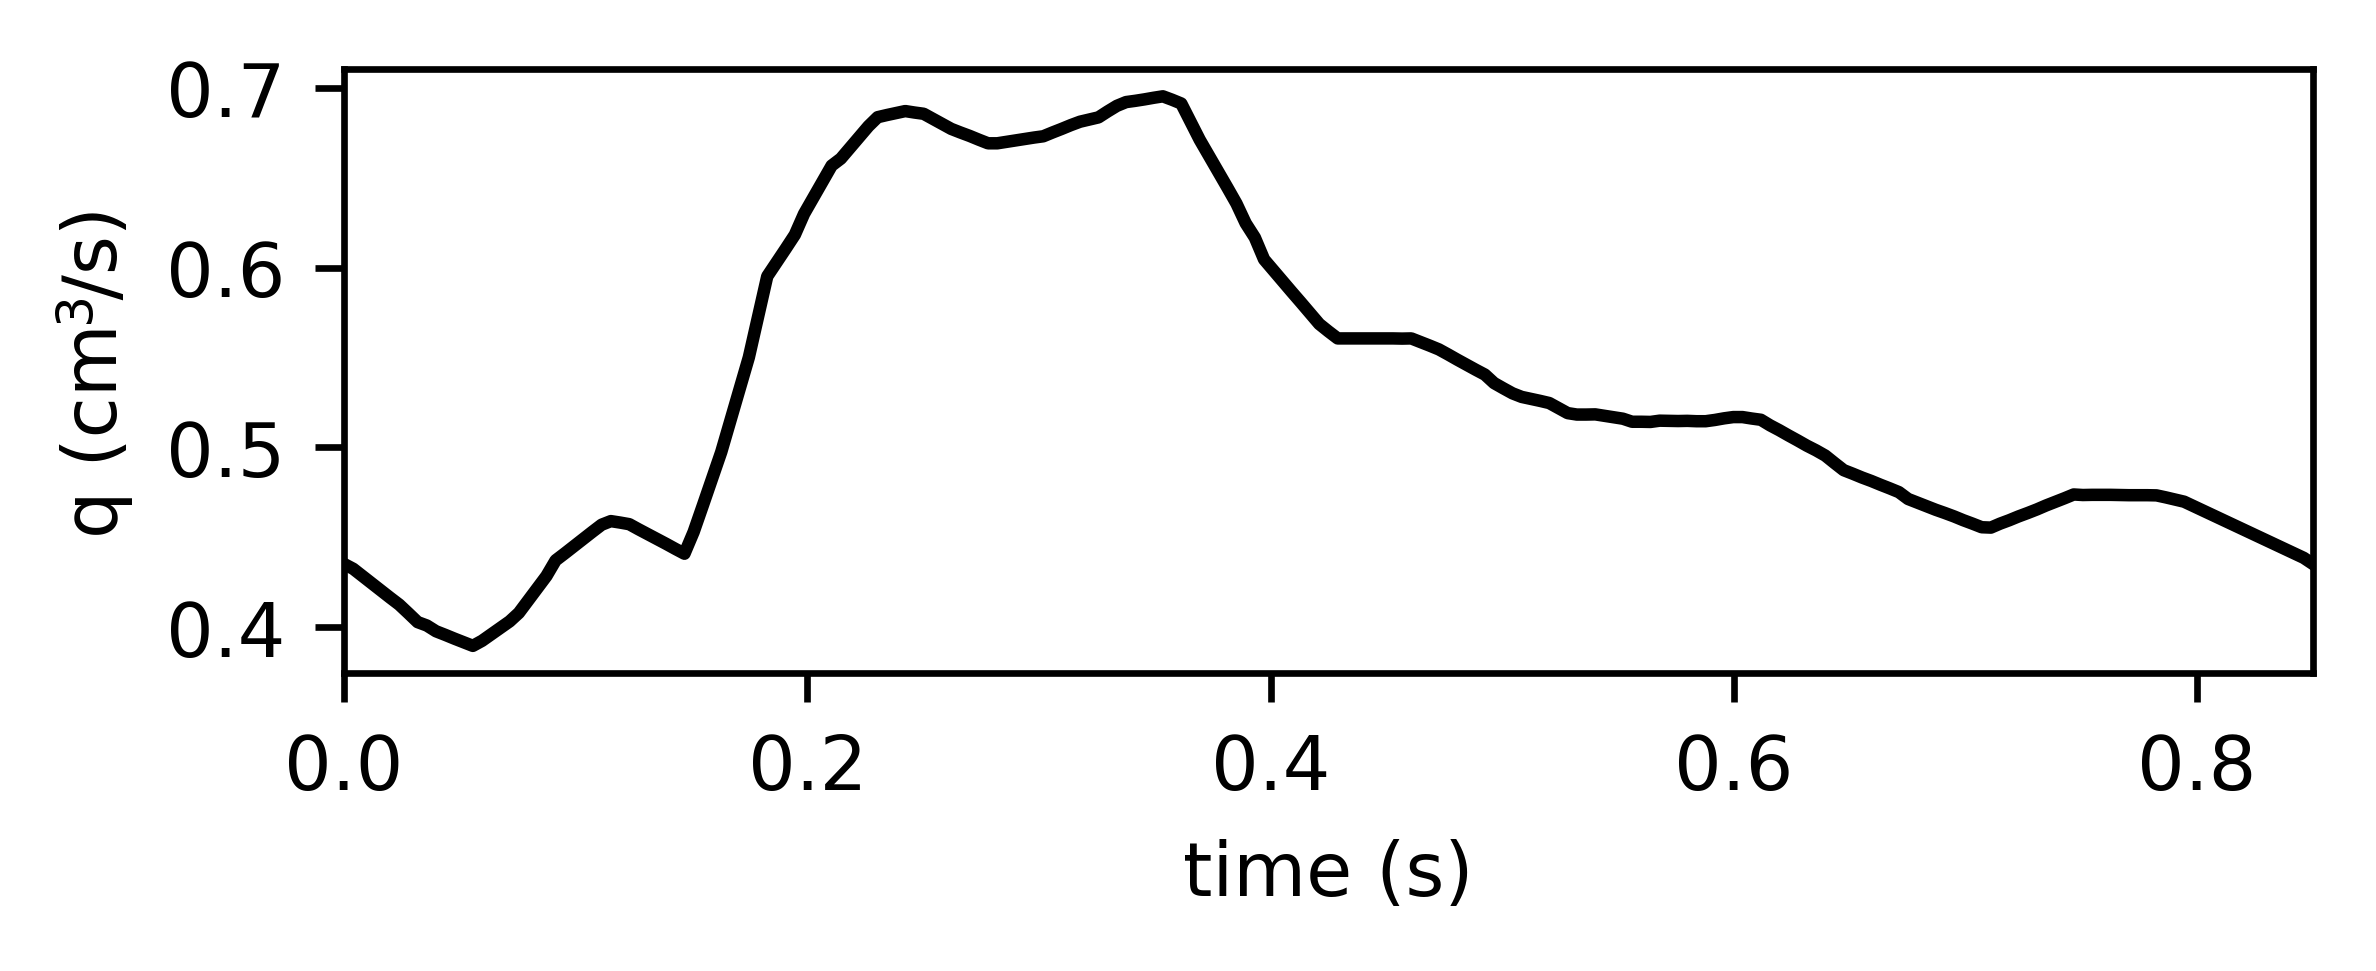
\includegraphics[width=10cm]{figures/inlet.png}
\textbf{\refstepcounter{figure}\label{fig:inlet} Figure \arabic{figure}.}{Inlet function for MCA simulations obtained from patient-specific measurements used to represent one period of \SI{0.85}{\second} of the pulse wave. The final ten peaks of the velocity time series were averaged in the Fourier space and adjusted such that its range of values aligns with those reported in \cite{Olufsen2002}. The resulting inlet function is smooth and serves as the inlet boundary condition for the MCA simulations using VaMpy \cite{Diem2016a}.}
\end{figure}

\begin{figure}[h!]
\centering
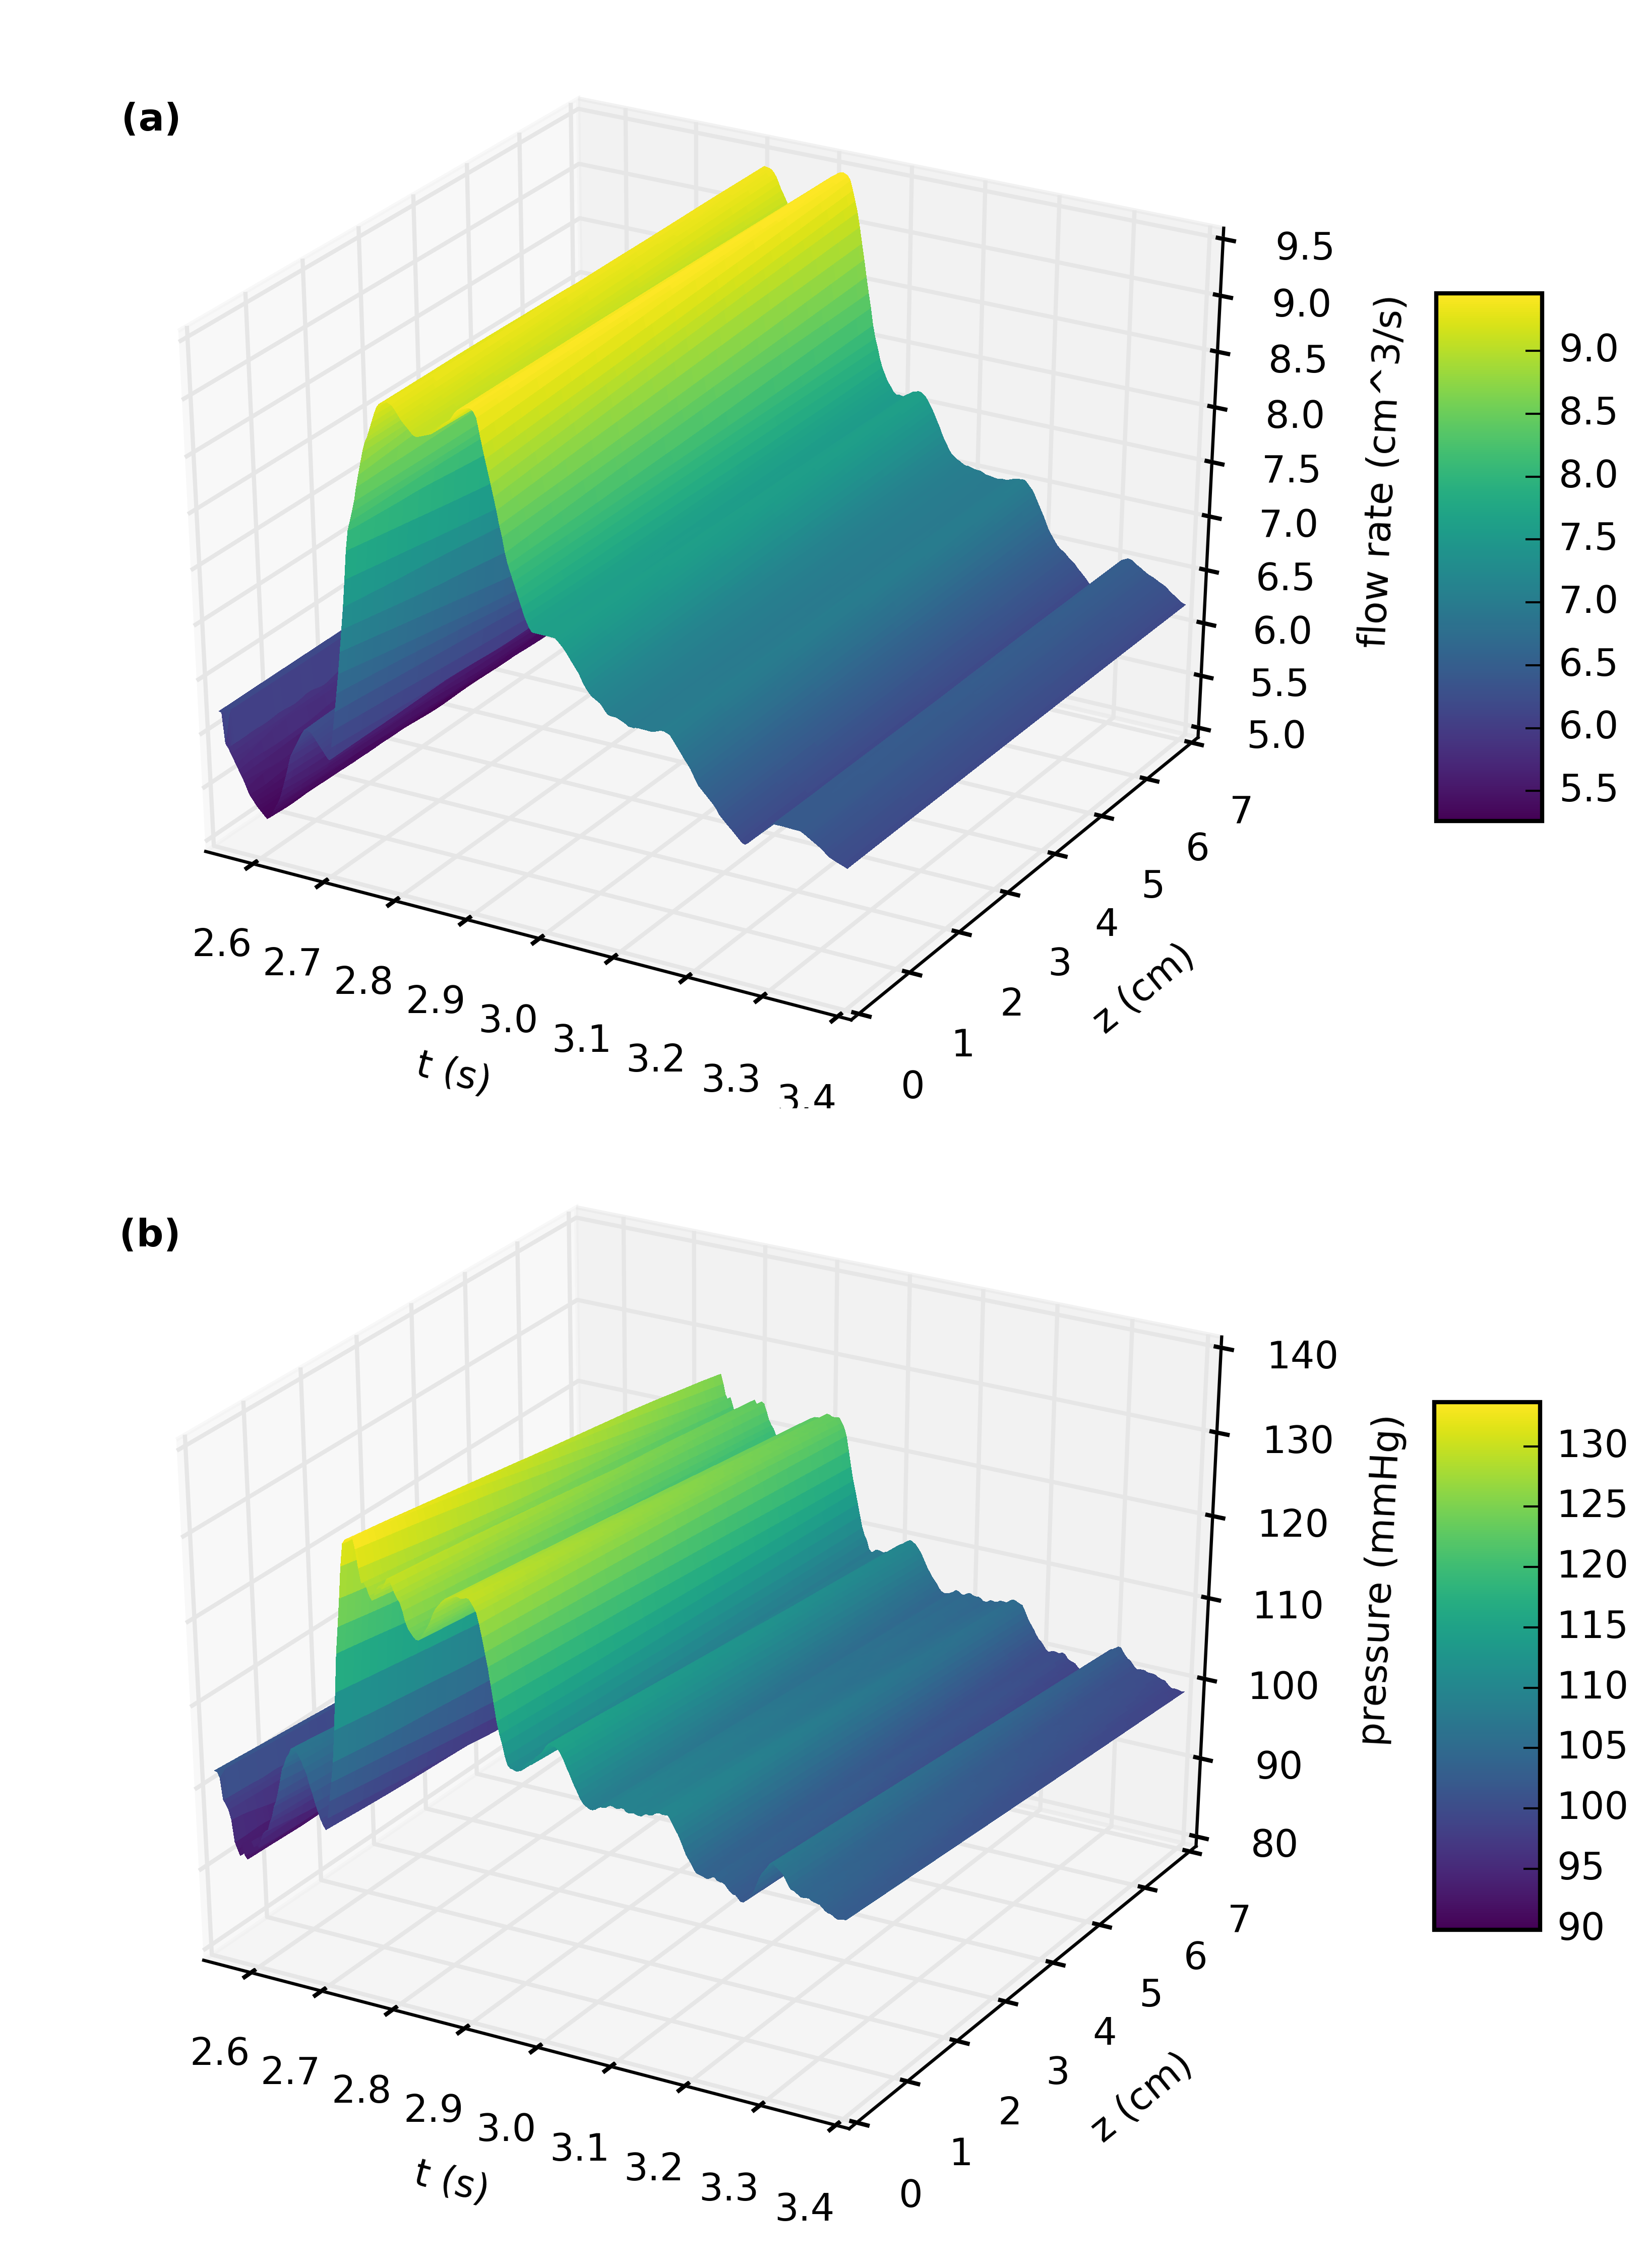
\includegraphics[width=10cm]{figures/mca.pdf}
\textbf{\refstepcounter{figure}\label{fig:mca} Figure \arabic{figure}.}{Blood pressure (a), wall displacement (b) and the resulting ISF pressure (c) in the MCA. Simulations were performed using the VaMpy Python package \cite{Diem2016a} and the simulation parameters are listed in Table~\ref{tab:simulation}. Wall stiffness is high in small blood vessels, therefore pressure gradients in time are steep. Wall displacement was calculated from the linear elasticity approximation derived in SI~2. The input function $R_i(z,t)$ to the BM model equation \eqref{eq:pvs_model} is obtained by adding the radius at rest $a$ (see geometry depiction in Figure~\ref{fig:pvs_model}).}
\end{figure}

\begin{figure}[h!]
\centering
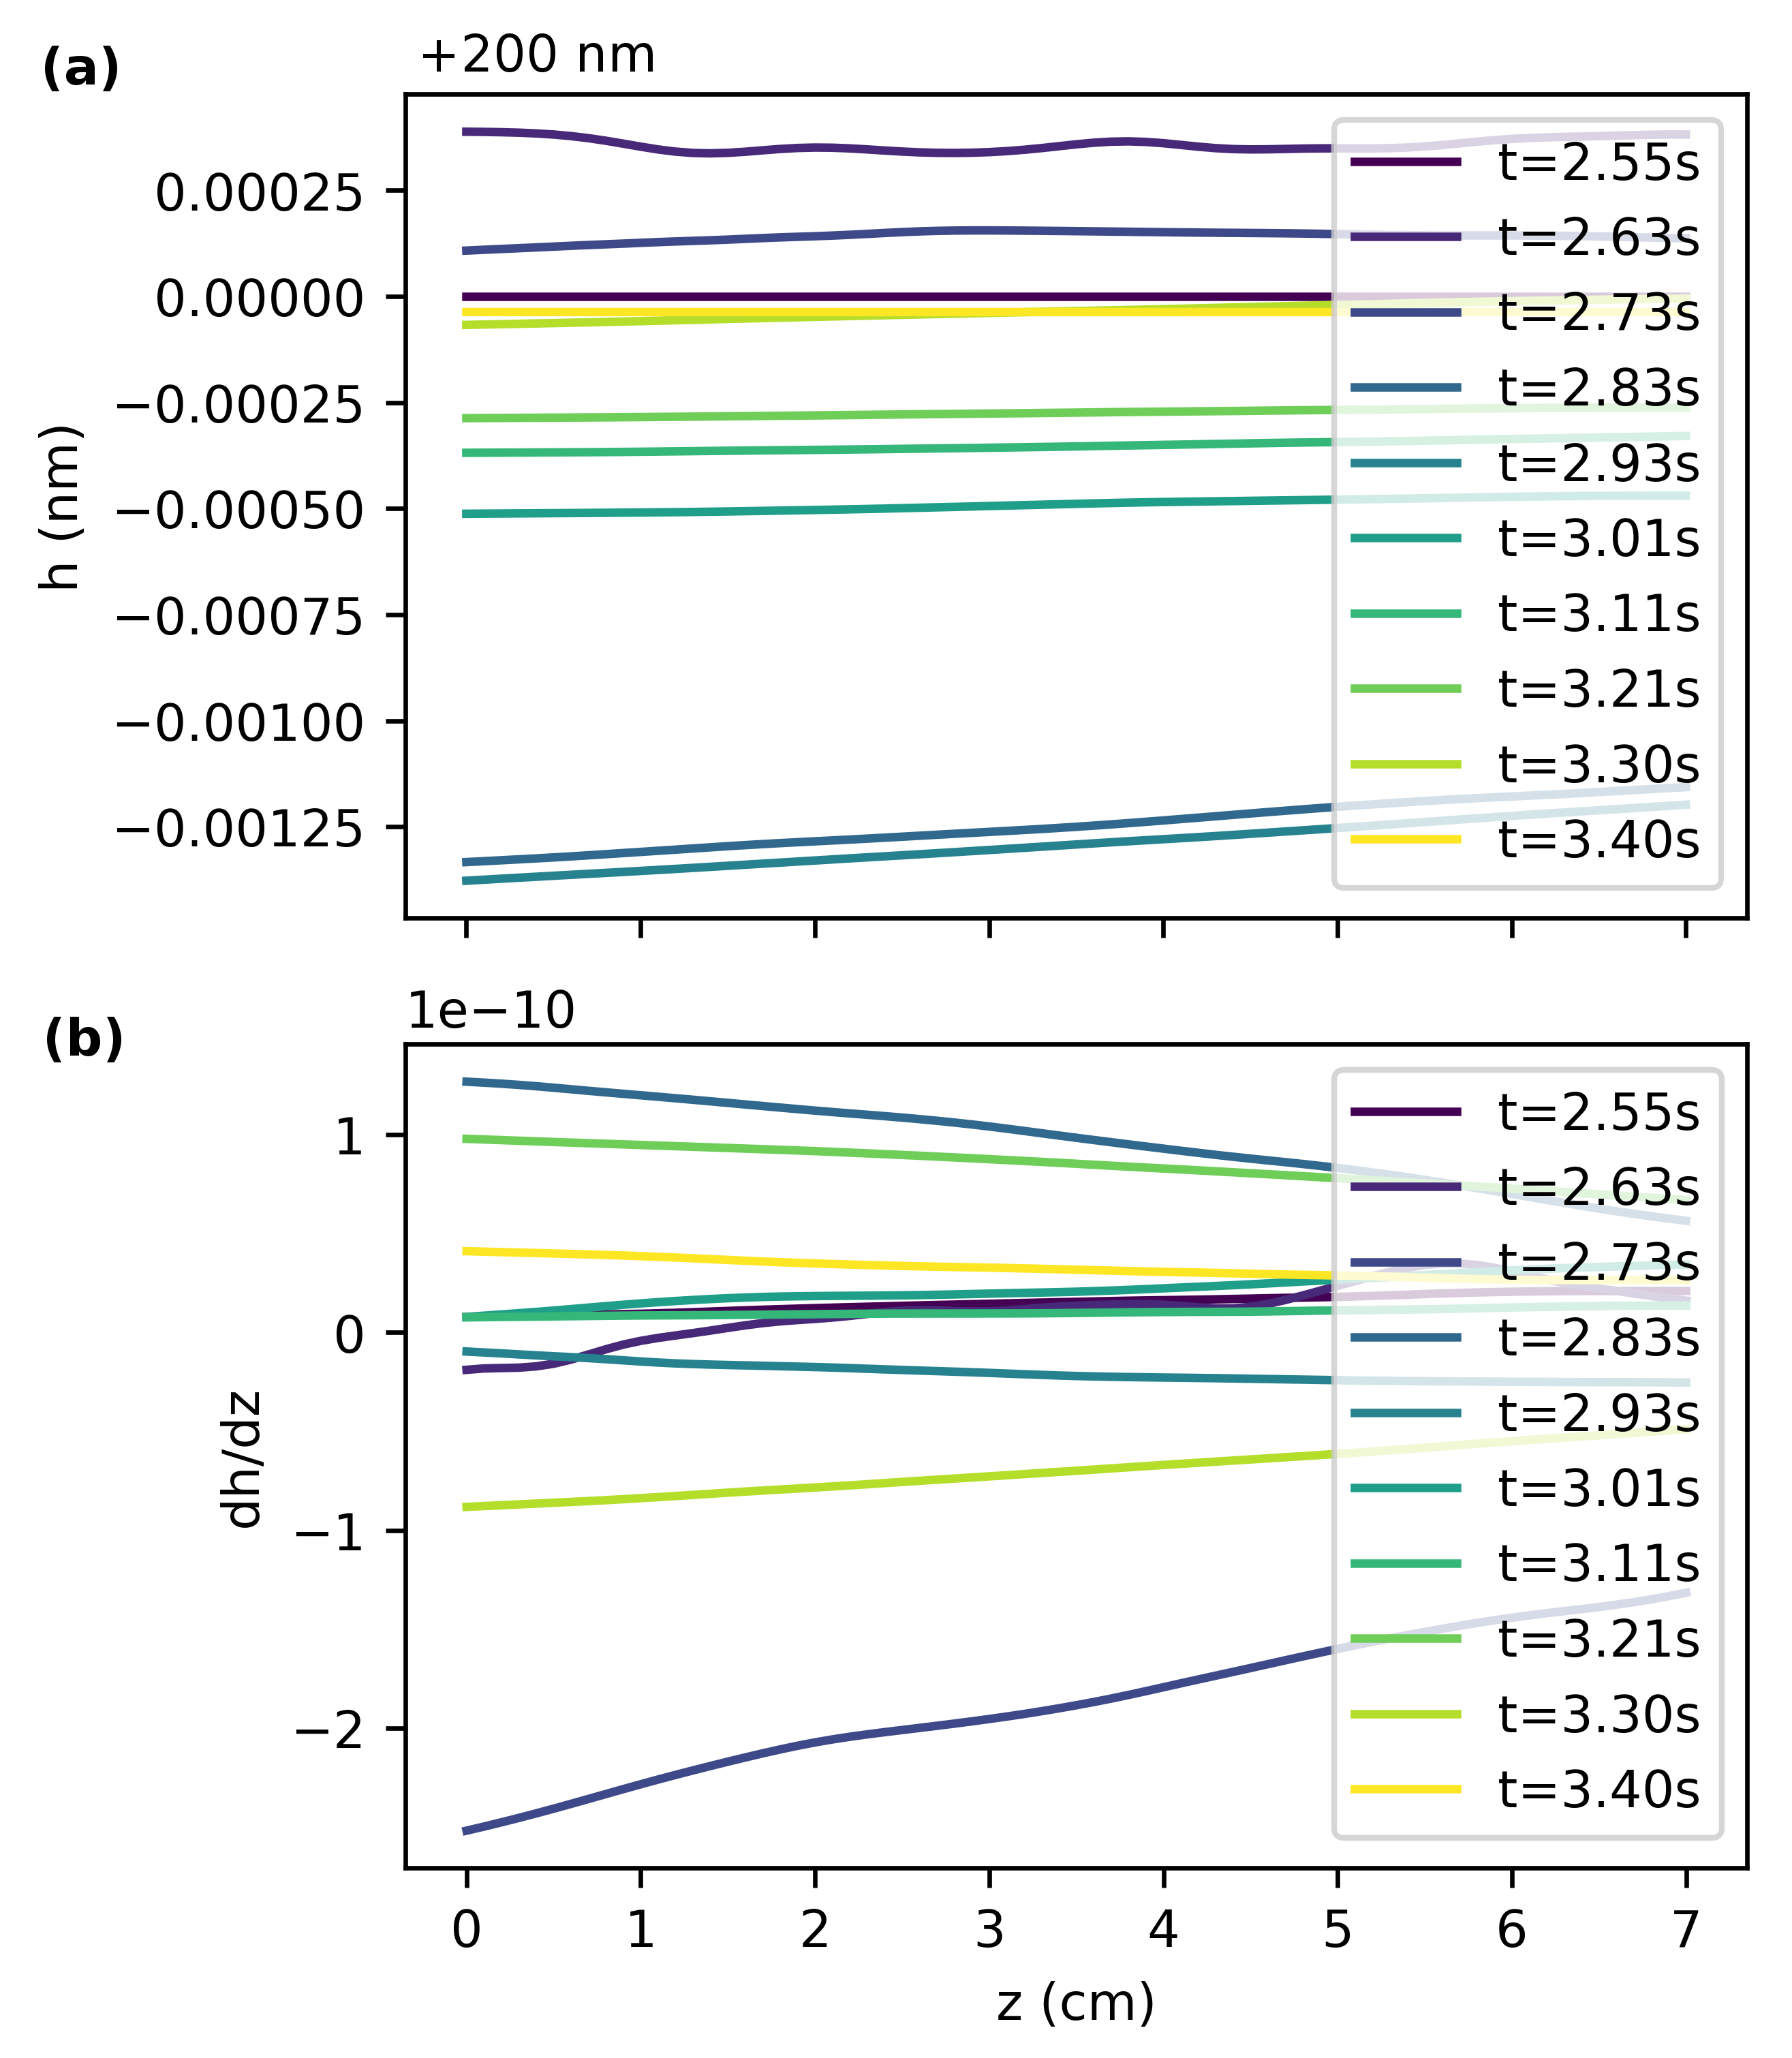
\includegraphics[width=10cm]{figures/h_dh.png}
\textbf{\refstepcounter{figure}\label{fig:h} Figure \arabic{figure}.}{BM width $h_\textrm{bm}(z,t)$ at several time points during the cardiac cycle (a) and its gradient along the $z$-axis at the same time points (b). Pressure pulse driven variations of the BM width are small compared to the initial width of \SI{200}{\nano\metre} and thus flow through the BM is slow.}
\end{figure}

\begin{figure}[h!]
\centering
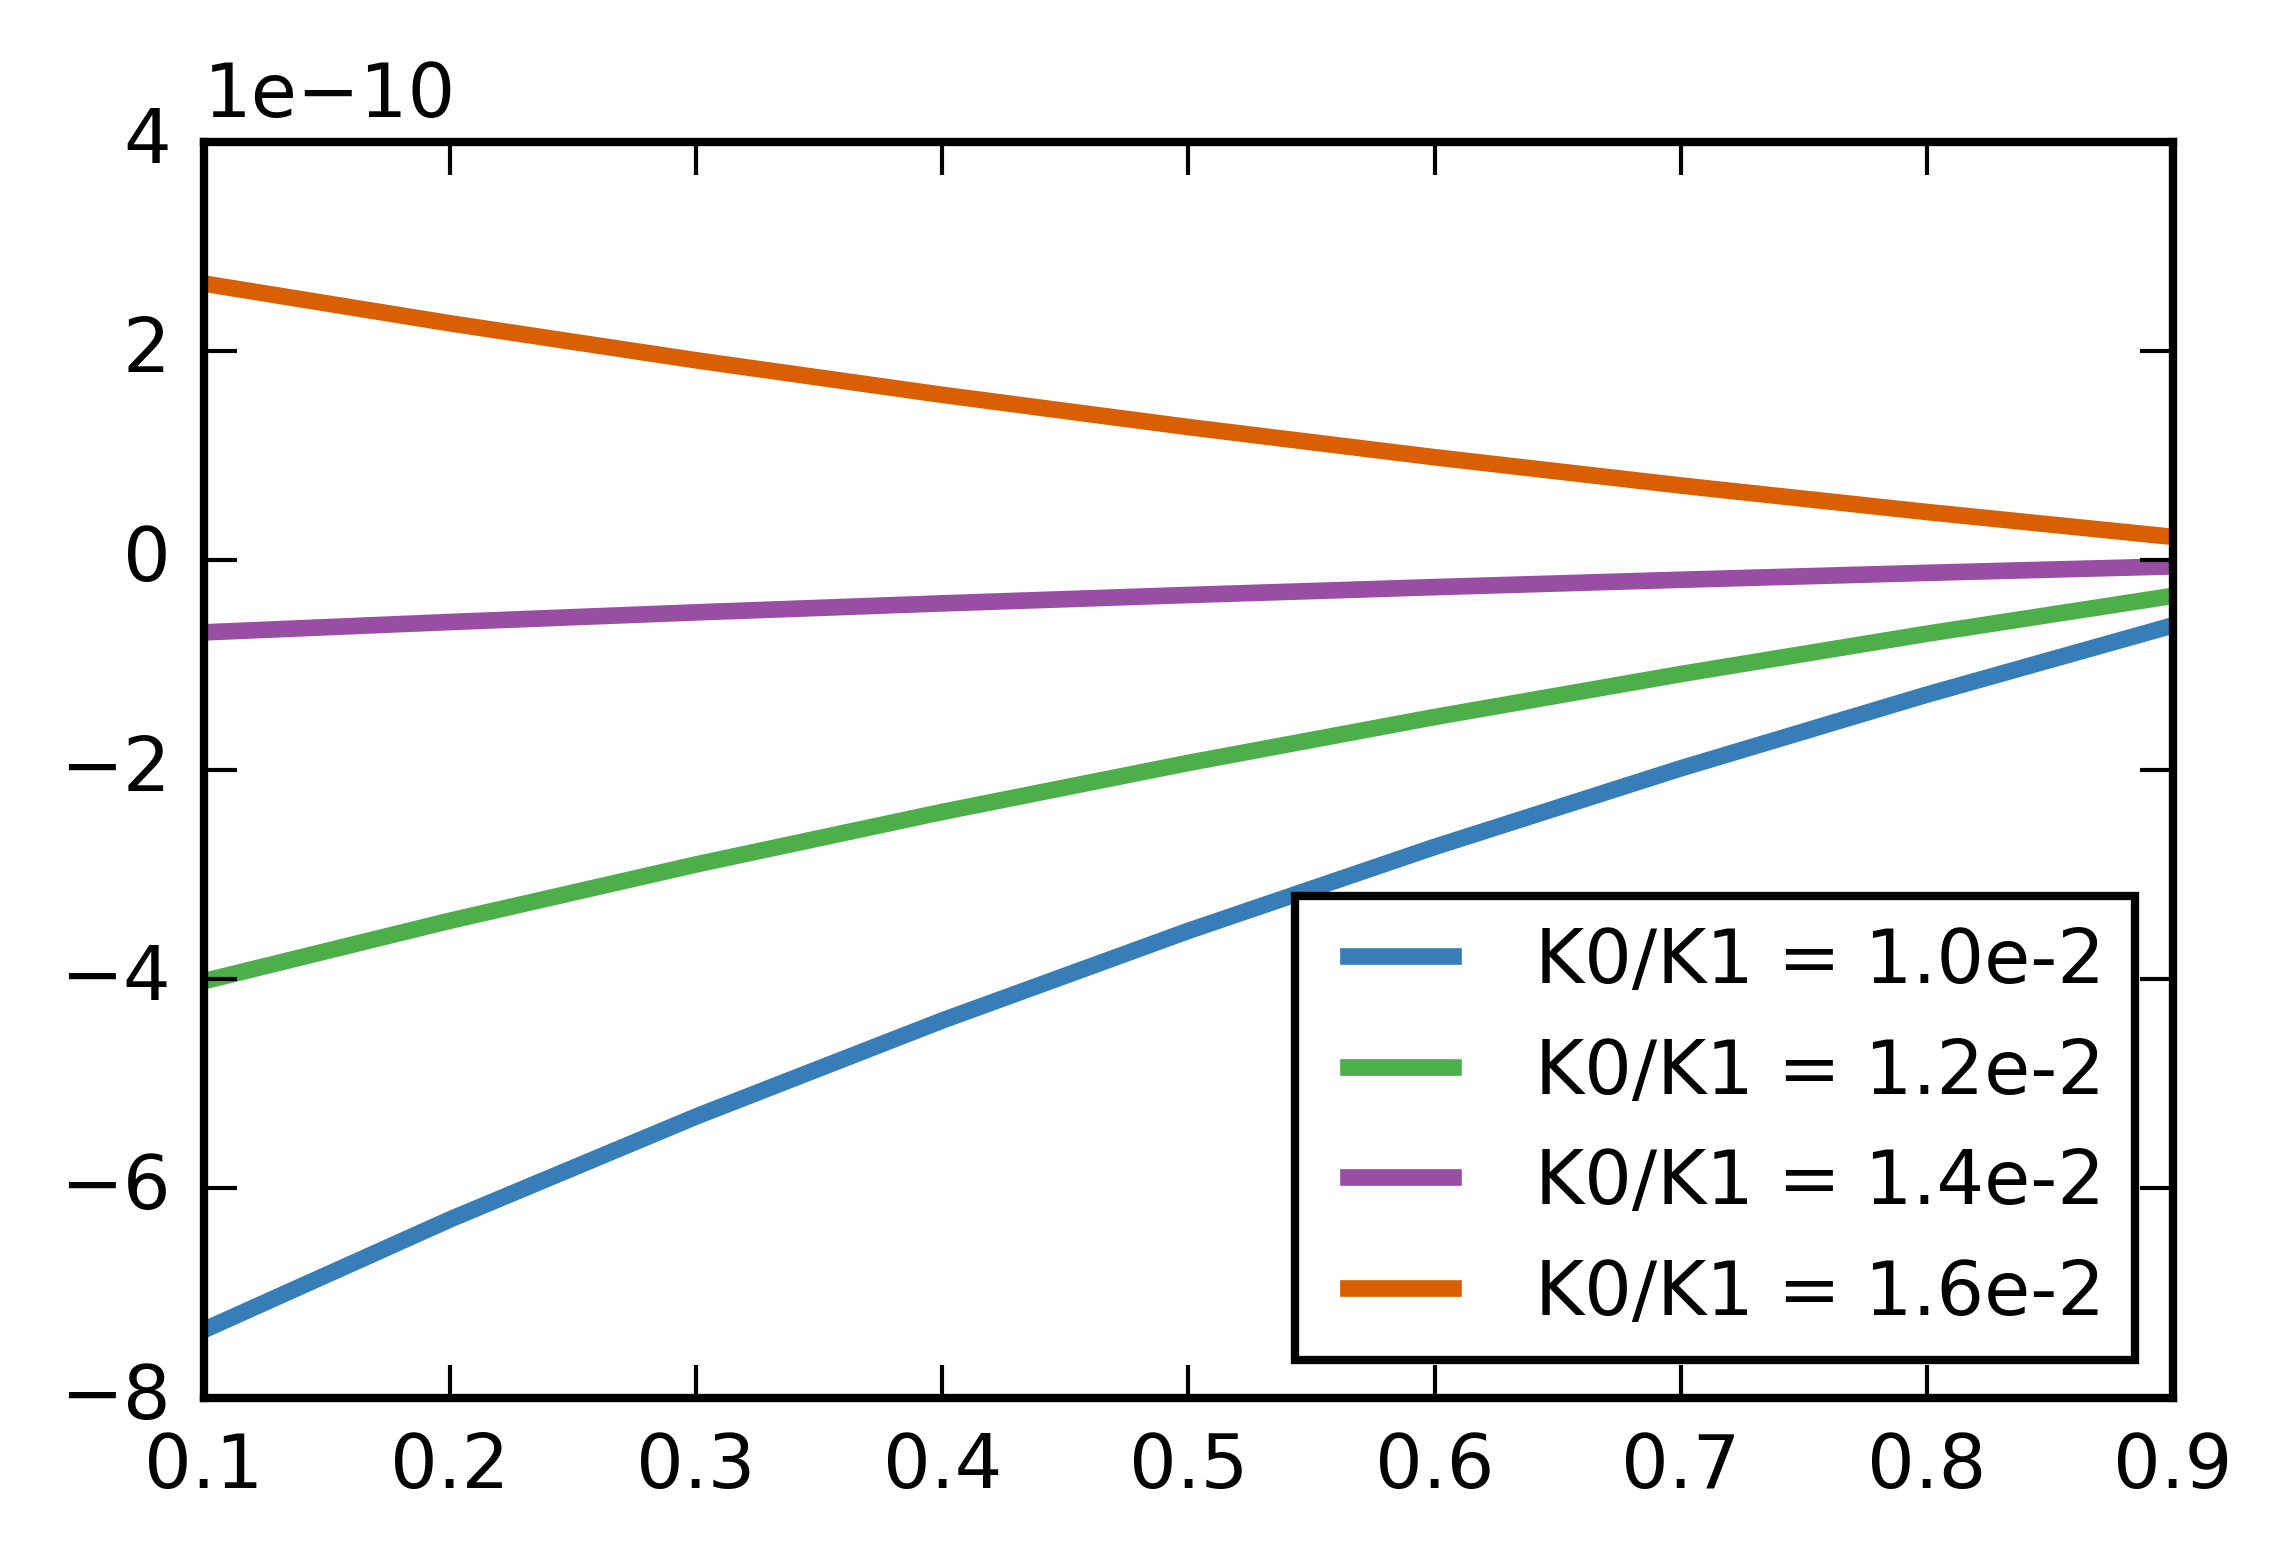
\includegraphics[width=10cm]{figures/valve_test.png}
\textbf{\refstepcounter{figure}\label{fig:valve_test} Figure \arabic{figure}.}{ISF flux (positive values in the direction of arterial flow) averaged over one cycle as a function of BM position $\eta$ in the arterial wall. Here the BM is at $r = r_0 + \eta h$ such that $\eta = 0$ represents a BM immediately adjacent to the lumen and $\eta = 1$ represents a BM on the outer wall of the artery. Note that reverse flow is only achieved by ratios of $K_0/K_1 < \SI{2.74e-2}{}$. The fastest net reverse drainage shown here (for $K_0/K_1 = \SI{2.68e-2}{}$ and on the arterial lumen $\eta = 0$) is \SI{-2.64e-5}{\cubic\micro\metre\per\second}.}
\end{figure}

\begin{figure}[h!]
\centering
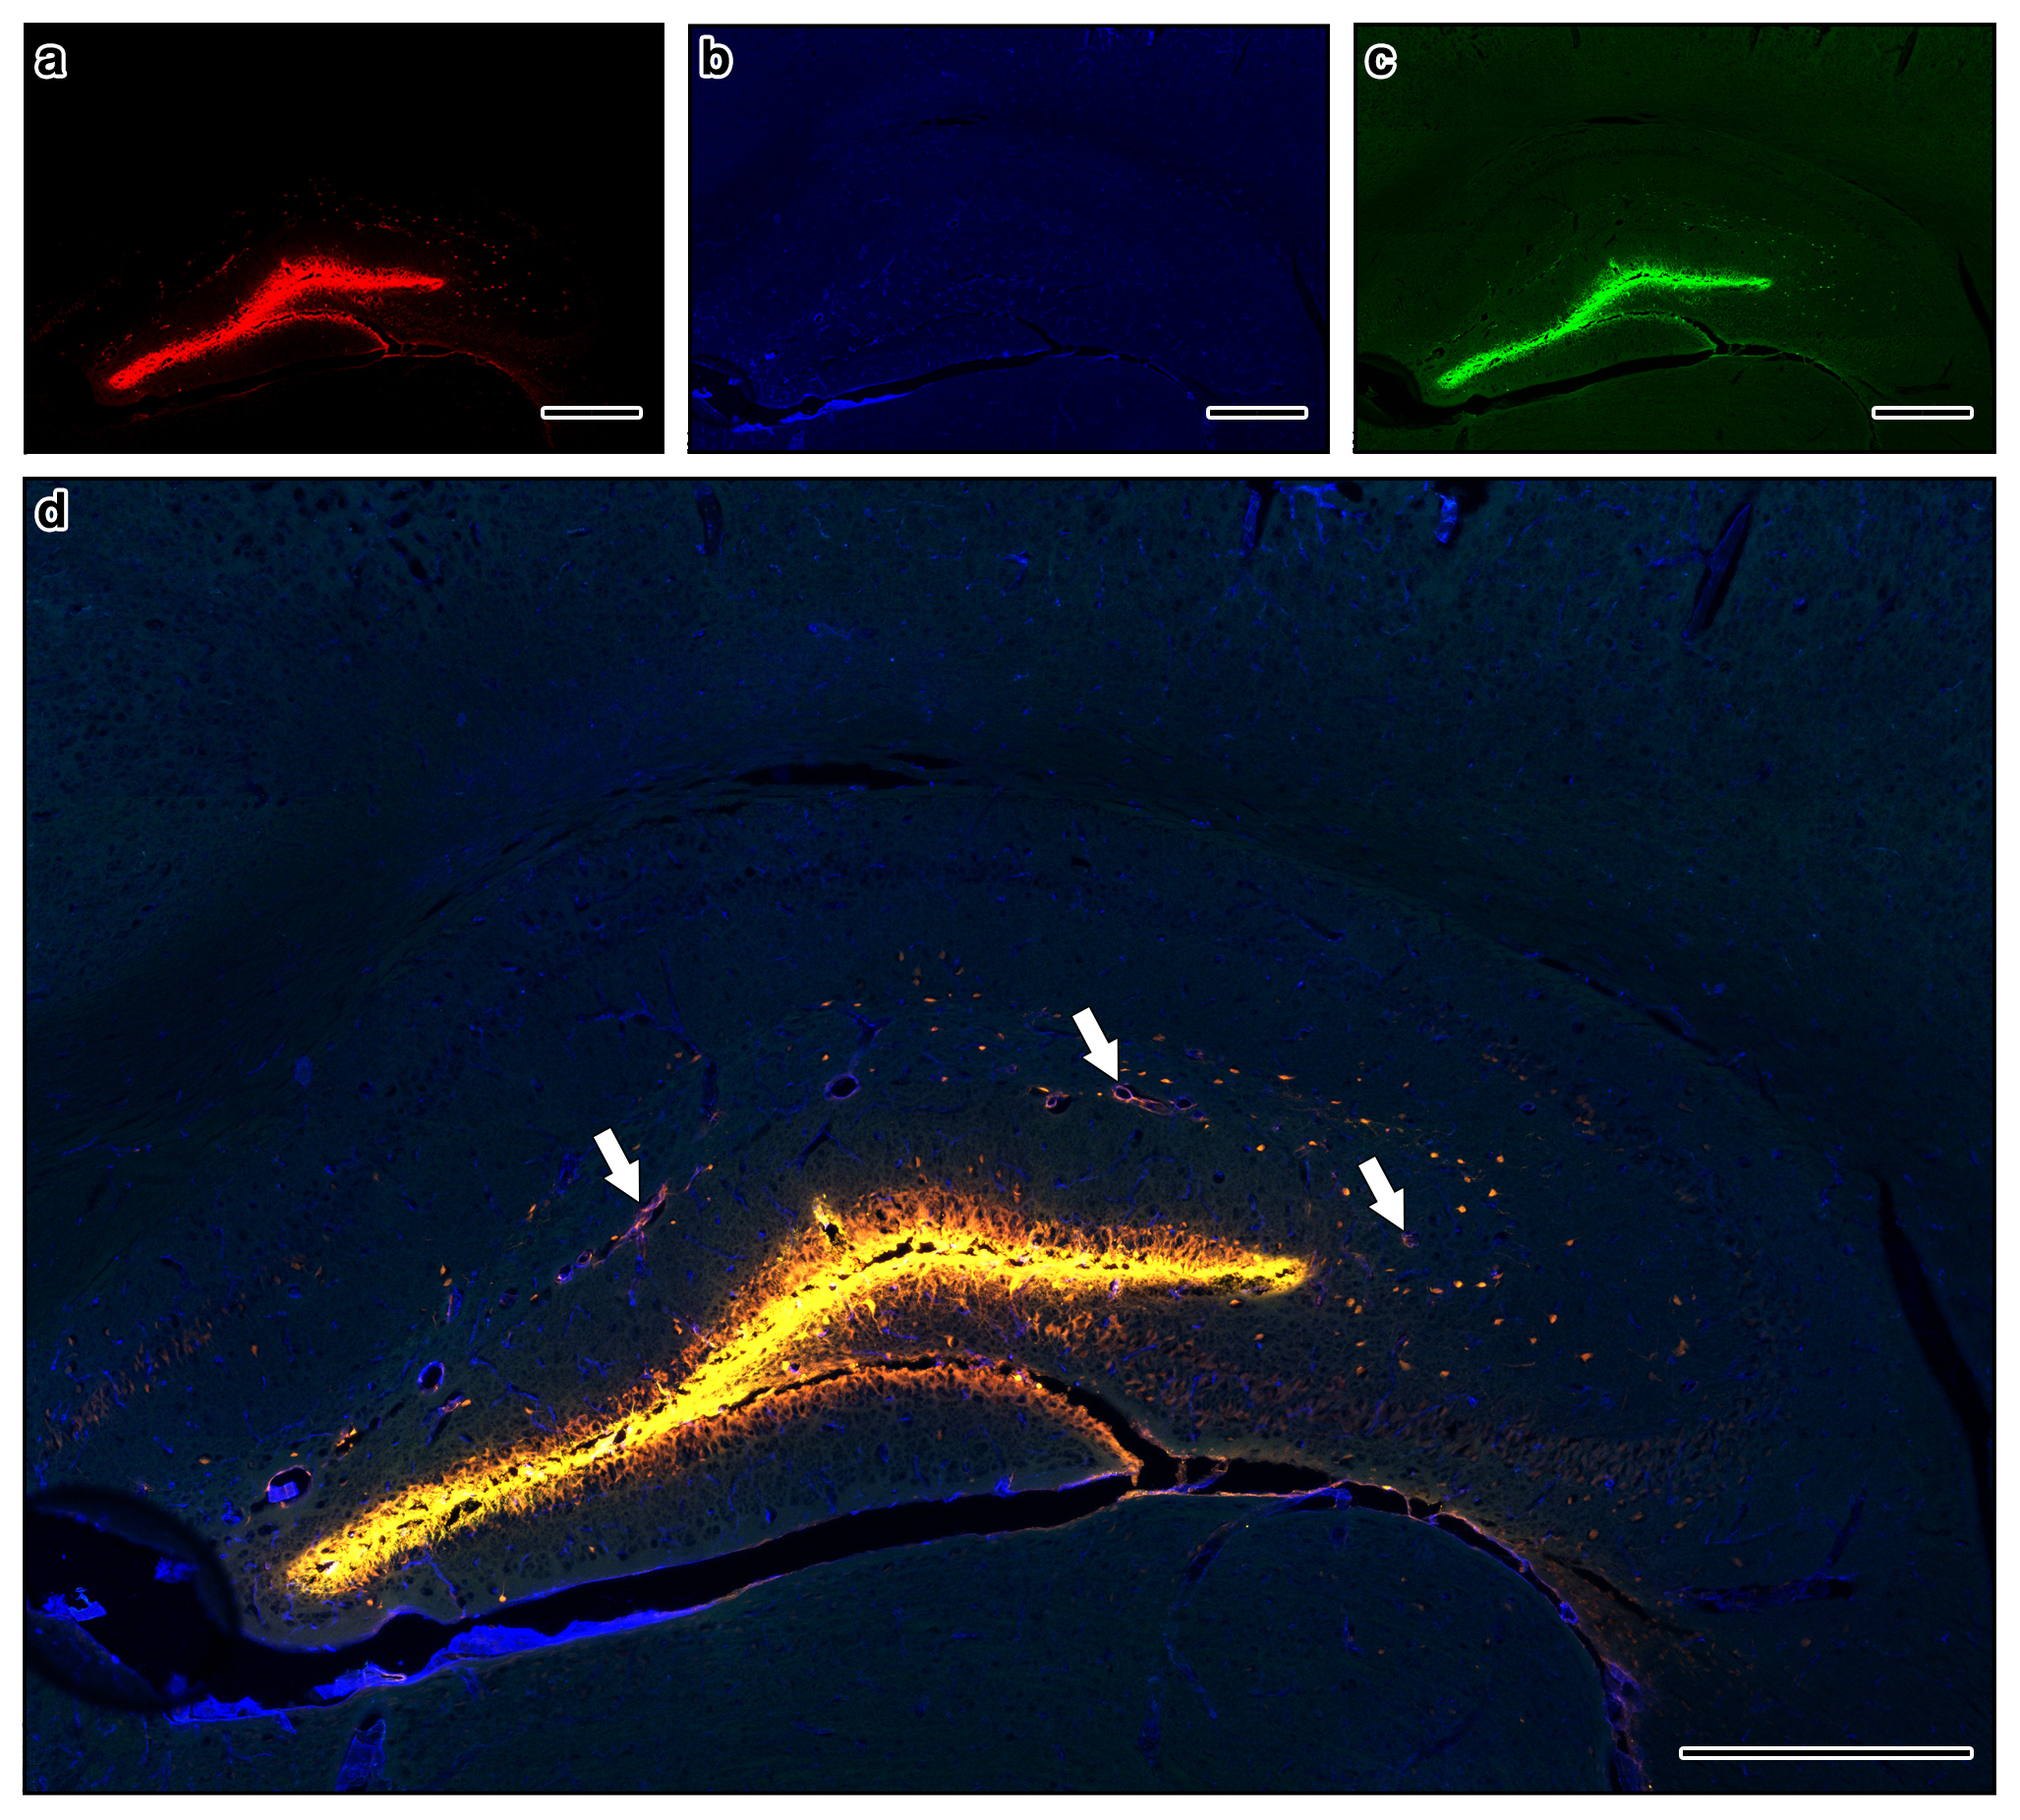
\includegraphics[width=10cm]{figures/confocal.jpg}
\textbf{\refstepcounter{figure}\label{fig:confocal} Figure \arabic{figure}.}{Composite tile scan of confocal images of the distribution of intracerebrally injected \Ab, in relation to collagen IV and SMA. Immunostaining \Ab: red, SMA: green, collagen IV: blue. Arrows are pointing to arteries with \Ab in the intramural perivascular drainage pathways.}
\end{figure}

\begin{figure}[h!]
\centering
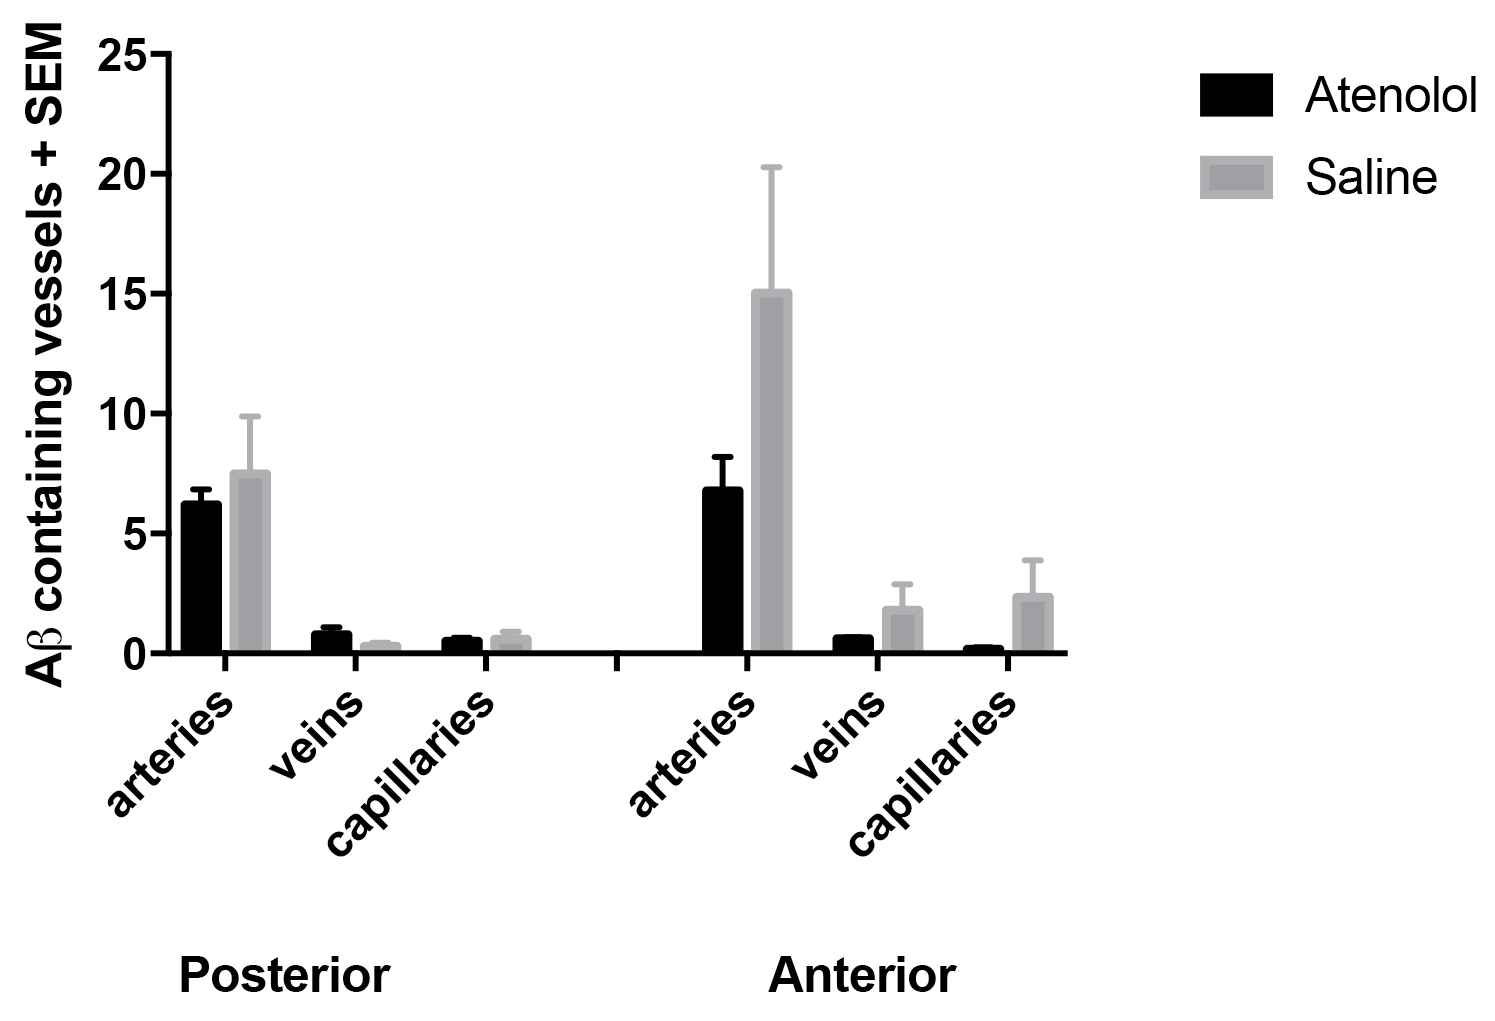
\includegraphics[width=10cm]{figures/graph.png}
\textbf{\refstepcounter{figure}\label{fig:graph} Figure \arabic{figure}.}{Graphs showing the number of arteries, veins and capillaries with \Ab in their walls in atenolol treated mice compared to control mice. SEM: standard error of mean.}
\end{figure}

%%% If you don't add the figures in the LaTeX files, please upload them when submitting the article.

%%% Frontiers will add the figures at the end of the provisional pdf automatically %%%

%%% The use of LaTeX coding to draw Diagrams/Figures/Structures should be avoided. They should be external callouts including graphics.

\end{document}
